\chapter{Genetic Drift and Neutral Diversity}
\label{Chapter:Drift}
\newthought{Randomness is inherent to evolution}, from the lucky birds blown of course to colonize some new oceanic island, to which mutations arise first in the HIV strain infecting an individual taking anti-retroviral drugs. One major source of stochasticity in evolutionary biology is genetic drift.  Genetic drift occurs because more or less copies of an allele by chance can be transmitted to the next generation. This can occur because, by chance, the individuals carrying a particular allele can leave more or less offspring in the next generation. In a
sexual population, genetic drift also occurs because Mendelian transmission
means that only one of the two alleles in an individual, chosen at random at a
locus, is transmitted to the offspring.

Genetic drift can play a role in the dynamics of all alleles in all populations, but it will play the biggest role for neutral alleles. A neutral polymorphism occurs when the segregating alleles at a polymorphic site have no discernible differences in their effect on fitness. We'll make clear what we mean by "discernible" later, but for
the moment think of this as "no effect" on fitness.
\paragraph{The neutral theory of molecular evolution.}
The role of genetic drift in molecular evolution has been hotly debated since the 60s when the Neutral theory of molecular evolution was proposed \citep[see ][ for a history]{ohta1996development}\cite{kimura:68,king:69,kimura:83}.  The central premise of Neutral theory theory is that patterns of molecular polymorphism within species and substitution between species can be well understood by supposing that the vast majority of these molecular polymorphisms and substitutions were neutral alleles, whose dynamics were just subject to the vagaries of genetic drift and mutation. Early proponents of this view suggested that the vast majority of new mutations are either neutral or highly deleterious (e.g. mutations that disrupt important protein functions). This latter class of mutations are too deleterious to contribute much to common polymorphisms or substitutions between species, because they are quickly weeded out of the population by selection.

Neutral theory can sound strange given that much of the time our first brush with evolution often focuses on adaptation and phenotypic evolution. However, proponents of this world-view didn't deny the existence of advantageous mutations, they simply thought that beneficial mutations are rare enough that their contribution to the bulk of polymorphism or divergence can be largely ignored. They also often thought that much of phenotypic evolution may well be adaptive, but again the loci responsible for these phenotypes are a small fraction of all the molecular change that occur. The neutral theory of molecular evolution was originally proposed to explain protein polymorphism. However, we can apply it more broadly to think about neutral evolution genome-wide. With that in mind, what types of molecular changes could be neutral? Perhaps:
\begin{enumerate}
\item Changes in non-coding DNA that don't disrupt regulatory sequences. For example, in the human genome only about 2\% of the genome codes for proteins. The rest is mostly made up of old transposable element and retrovirus insertions, repeats, pseudo-genes, and general genomic clutter. Current estimates suggest that, even counting conserved, functional, non-coding regions, less than 10\% of our genome is subject to evolutionary constraint \citep{rands:14}.
\item Synonymous changes in coding regions, i.e. those that don't change the amino-acid encoded by a codon.
\item Non-synonymous changes that don't have a strong effect on the functional properties of the amino acid encoded, e.g. changes that don't change the size, charge, or hydrophobic properties of the amino acid too much.
\item An amino-acid change with phenotypic consequences, but little relevance to fitness, e.g. a mutation that causes your ears to be a slightly different shape, or that prevents an organism from living past 50 in a species where most individuals reproduce and die by their 20s.
\end{enumerate}
There are counter examples to all of these ideas, e.g. synonymous changes can affect the translation speed and accuracy of proteins and so are subject to selection. However, the list above hopefully convinces you that the general thinking that some portion of molecular change may not be subject to selection isn't as daft as it may have initially sounded.

Various features of molecular polymorphism and divergence have been viewed as consistent with the neutral theory of molecular evolution. The two we'll focus on in this chapter are the high level of molecular polymorphism in many species (see for example Figure \ref{fig:Leffer}) and the molecular clock. We'll see that various aspects of the original neutral theory have merit in describing some features and types of molecular change, but we'll also see that it is demonstrably wrong in some cases. We'll also see the primary utility of the neutral theory isn't whether it is right or wrong, but that it serves as a simple null model that can be tested and in some cases rejected, and subsequently built on. The broader debate currently in the field of molecular evolution is the balance of neutral, adaptive, and deleterious changes that drive different types of evolutionary change.

\section{Loss of heterozygosity due to drift.} \label{LossofHet}

Genetic drift will, in the absence of new mutations, slowly purge our population of neutral genetic diversity, as alleles slowly drift to high or low
frequencies and are lost or fixed over time. \\

Imagine a randomly mating population of a constant size $N$ diploid individuals, and that we
are examining a locus segregating for two alleles that are neutral with respect
to each other.  This population is randomly mating with respect to the alleles
at this locus. See Figures \ref{fig:LossHet_two_alleles} and
\ref{fig:LossHet_many_alleles} to see how genetic drift proceeds, by tracking
alleles within a small population. \\


In generation $t$ our current level of heterozygosity is $H_t$,
i.e. the probability that two randomly sampled alleles in generation
$t$ are non-identical is $H_t$. Assuming that the mutation rate is
zero (or vanishingly small), what is our level of heterozygosity in
generation $t+1$?\\

\begin{figure}
\begin{center}
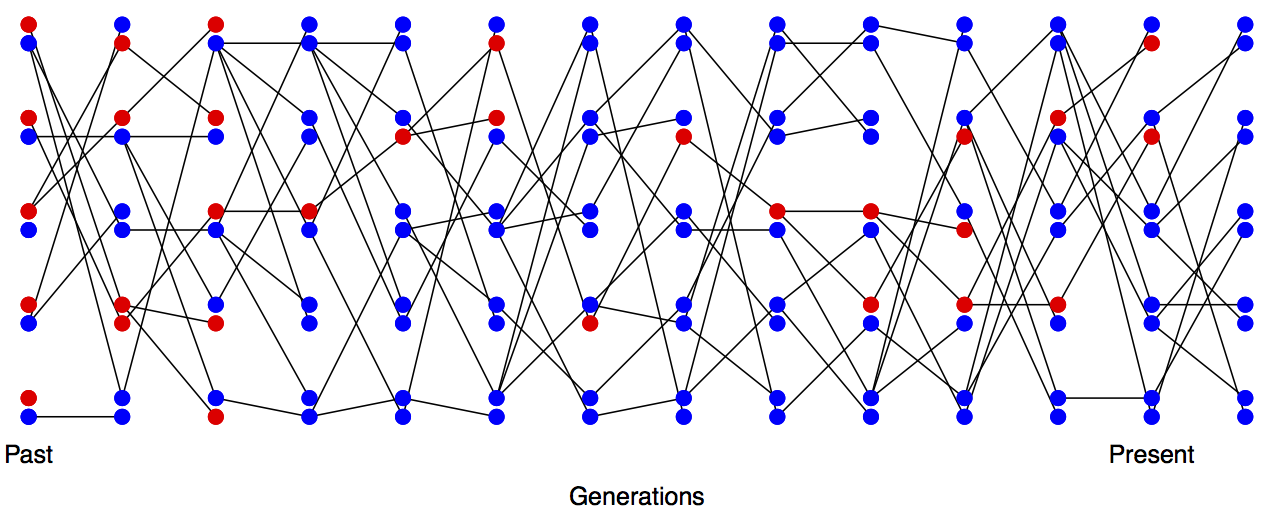
\includegraphics[width= \textwidth]{figures/Loss_of_he_col_two_alleles.png}
\end{center}
\caption{Loss of heterozygosity over time, in the absence of new
  mutations. A diploid population of 5 individuals over the
  generations, with lines showing transmission. In the first
  generation every individual is a heterozygote. \gitcode{https://github.com/cooplab/popgen-notes/blob/master/Rcode/Loss_of_heterozyg_varying_pop.R} } \label{fig:LossHet_two_alleles}
\end{figure}

\begin{figure}
\begin{center}
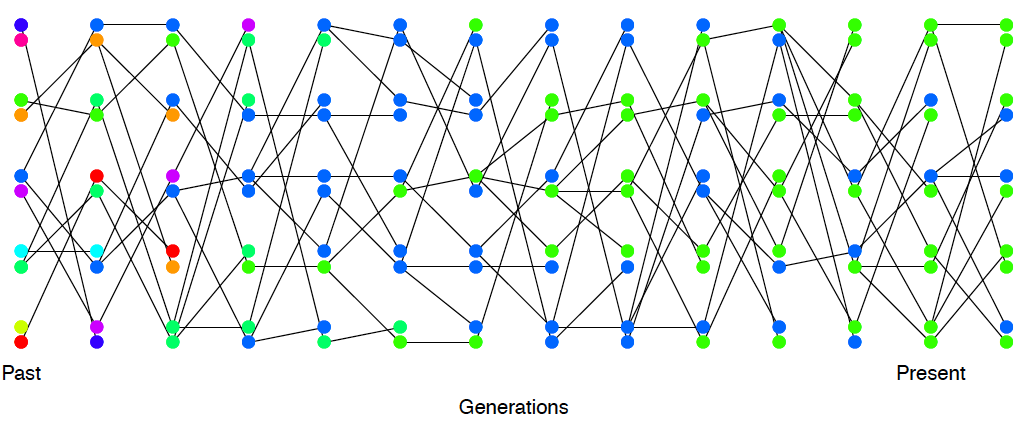
\includegraphics[width= \textwidth]{figures/Loss_of_het_2_many_alleles.png}
\end{center}
\caption{Loss of heterozygosity over time, in the absence of new
  mutations. A diploid population of 5 individuals. In the first generation I colour every allele a different
colour so we can track their descendants. \gitcode{https://github.com/cooplab/popgen-notes/blob/master/Rcode/Loss_of_heterozyg_varying_pop.R} } \label{fig:LossHet_many_alleles}
\end{figure}


In the next generation ($t+1$) we are looking at the alleles in the
offspring of generation $t$. If we randomly sample two alleles in generation
$t+1$ which had different parental alleles in generation $t$, that
is just like drawing two random alleles from generation $t$. So the
probability that these two alleles in generation $t+1$, that have
different parental alleles in generation $t$, are non-identical is
$H_t$. \\

Conversely, if the two alleles in our pair had the same parental allele in
the proceeding generation (i.e. the alleles are identical by descent
one generation back) then these two alleles must be identical (as we
are not allowing for any mutation). \\



In a diploid population of size $N$ individuals there are $2N$ alleles. The
probability that our two alleles have the same parental allele in the
proceeding generation is $\nicefrac{1}{(2N)}$ and the probability that they have
different parental alleles is is $1-\nicefrac{1}{(2N)}$. So by the above
argument, the expected heterozygosity in generation $t+1$ is
%
\begin{equation}
H_{t+1} = \frac{1}{2N} \times 0 + \left(1-\frac{1}{2N} \right)H_t
\end{equation}
%
Thus, if the heterozygosity in generation $0$ is $H_0$, our
expected heterozygosity in generation $t$ is
%
\begin{equation}
H_t = \left(1-\frac{1}{2N} \right)^tH_0  \label{eqn:loss_het_discrete}
\end{equation}
%
i.e. the expected heterozygosity within our population is decaying
geometrically with each passing generation. If we assume that $\nicefrac{1}{(2N)}
\ll 1$ then we can approximate this geometric decay by an exponential
decay (see Question \ref{geo_question} below), such that
%
\begin{equation}
H_t =H_{0} e^{ - \nicefrac{t}{(2N)} }
\end{equation}
%
i.e. heterozygosity decays exponentially at a rate
$\nicefrac{1}{(2N)}$.

In Figure \ref{fig:LossHet_WF_N50} we show trajectories through time for 40 independently simulated loci drifting in a population of 50 individuals. Each population was started from a frequency of $30\%$. Some drift up and some drift down, eventually being lost or fixed from the population, but, on average across simulations, the allele frequency doesn't change. We also track heterozygosity, you can see that heterozygosity sometimes goes up, and sometimes goes down, but on average we are losing heterozygosity, and this rate of loss is well predicted by eqn. \eqref{eqn:loss_het_discrete}.
\begin{figure}
\begin{center}
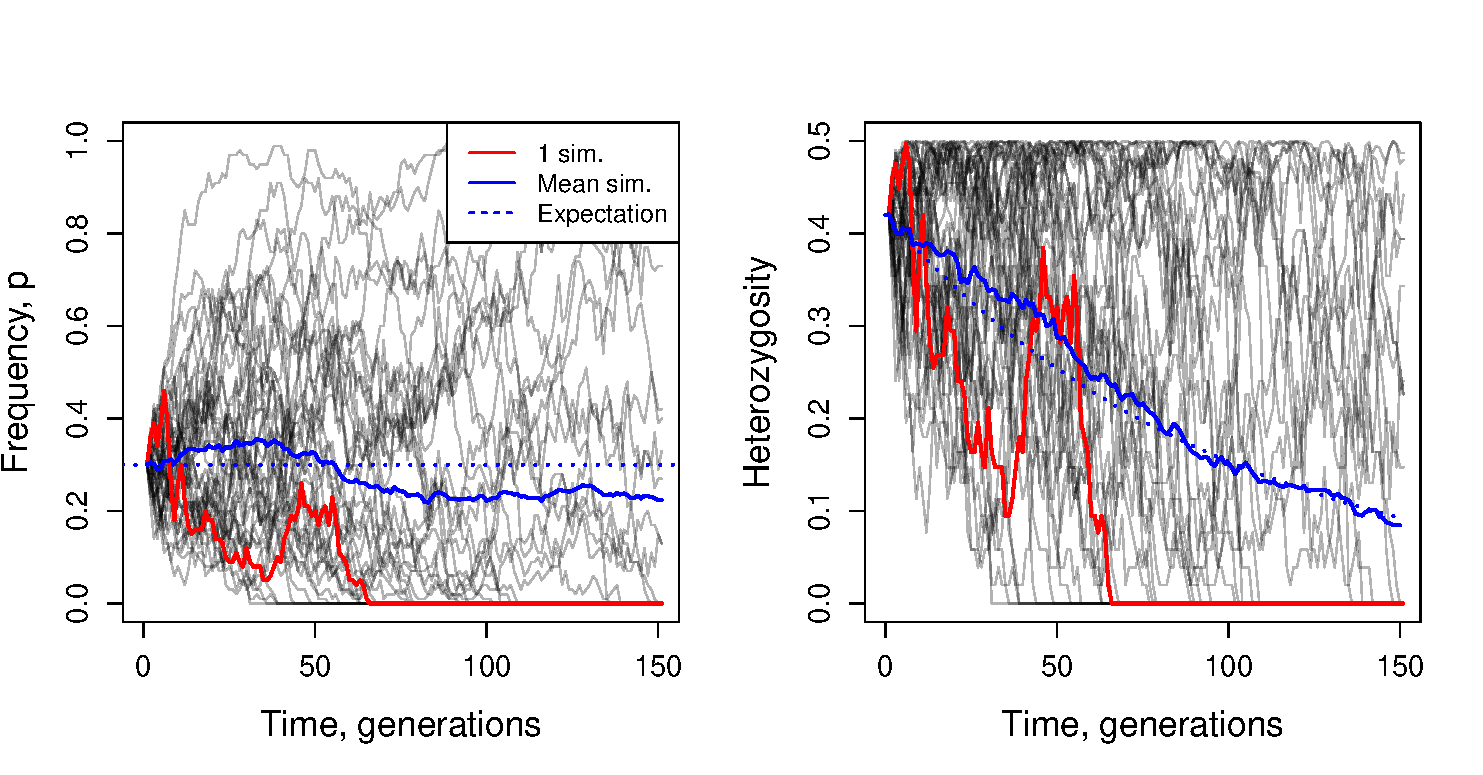
\includegraphics[width= \textwidth]{figures/WF_loss_het/WF_loss_het_N50.pdf}
\end{center}
\caption{Change in allele frequency and loss of heterozygosity over time for 40 replicates. Simulations of genetic drift in a diploid population of 50 individuals, in the absence of new mutations. We start 40 independent, biallelic loci each with an initial allele at 30\% frequency. The left panel shows the allele frequency over time and the right panel shows the heterozygosity over time, with the mean decay matching eqn. \eqref{eqn:loss_het_discrete}. \gitcode{https://github.com/cooplab/popgen-notes/blob/master/Rcode/Genetic_drift/WF_loss_of_het.R}} \label{fig:LossHet_WF_N50}
\end{figure}


\begin{marginfigure}
\begin{center}
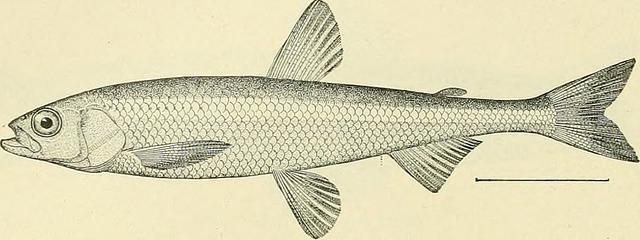
\includegraphics[width= \textwidth]{illustration_images/Genetic_drift/smelt/20497452375_9be855d9ff_z.jpg}
\end{center}
\caption{Pond smelt ({\it Hypomesus olidus}), a close relative of delta smelt. \BHLNC{Bulletin of the United States Fish Commission. 1906.}{https://archive.org/stream/bulletinofunited261906unit/\#page/270/mode/1up}{Smithsonian Libraries}} \label{fig:smelt}
\end{marginfigure}
%JRI: lame. i'd drop pic if you can't find one of right species.

\begin{question} You are in charge of maintaining a population of delta smelt in the Sacramento river delta. Using a large set of microsatellites you
  estimate that the mean level of heterozygosity in this population is 0.005.
  You set yourself a goal of maintaining a level of heterozygosity of at least
  0.0049 for the next two hundred years. Assuming that the smelt have a
  generation time of 3 years, and that only genetic drift affects these loci, what is the smallest fully outbreeding population that you would need to maintain to meet this goal?
\end{question}

Note how this picture of decreasing heterozygosity stands in contrast to the
consistency of Hardy-Weinberg equilibrium from the previous chapter.
%JRI: I don't recall discussion of HWE in previous chapter, just HW proportions.
However, our Hardy-Weinberg \emph{proportions} still hold in forming each new generation. As the offspring genotypes in the next generation ($t+1$) represent a random
draw from the previous generation ($t$), if the parental frequency is $p_t$, we \emph{expect} a proportion $2p_t(1-p_t)$ of our offspring to be
heterozygotes (and HW proportions for our homozygotes). However, because population size is finite, the
observed genotype frequencies in the offspring will (likely) not match exactly with our expectations. As our genotype frequencies likely change slightly due
to sampling, biologically this reflects random variation in family size
and Mendelian segregation, the allele frequency will changed. Therefore, while each generation represents a sample from
Hardy-Weinberg proportions based on the generation before, our
genotype proportions are not at an equilibrium (an unchanging state) as the
underlying allele frequency changes over the generations. We'll develop some mathematical models for these allele
frequency changes later on. For now, we'll simply note that
under our simple model of drift (formally the Wright-Fisher model), our
allele count in the $t+1^{th}$ generation represents a binomial sample
(of size $2N$) from the population frequency $p_t$ in the previous
generation.  If you've read to here, please email Prof Coop a picture of JBS Haldane in a striped suit with the title "I'm reading the chapter 3 notes''. (It's well worth googling JBS Haldane and to read more about his life; he's a true character and one of the last great polymaths. )

% generation $t$ may differ
%from that of $t+1$. We'll develop some mathematical models for these allele
%frequency changes
 %from the previous generation we are
%drawing alleles at random from the
%Here, the
%freqeuncy of each genotype will likely change, due to chance fluctuations in
%the underlying allele frequency $p$. While within a single generation
%Hardy--Weinberg proportions are maintained (at least approximately), across
%generations the genotypic frequencies change with allele frequency. The change
%in allele frequencies is due to drift: due to random variation in family size
%and Mendelian segregation, the allele frequency in generation $t$ may differ
%from that of $t+1$. We'll develop some mathematical models for these allele
%frequency changes later on.


\begin{marginfigure}[6cm]
\begin{center}
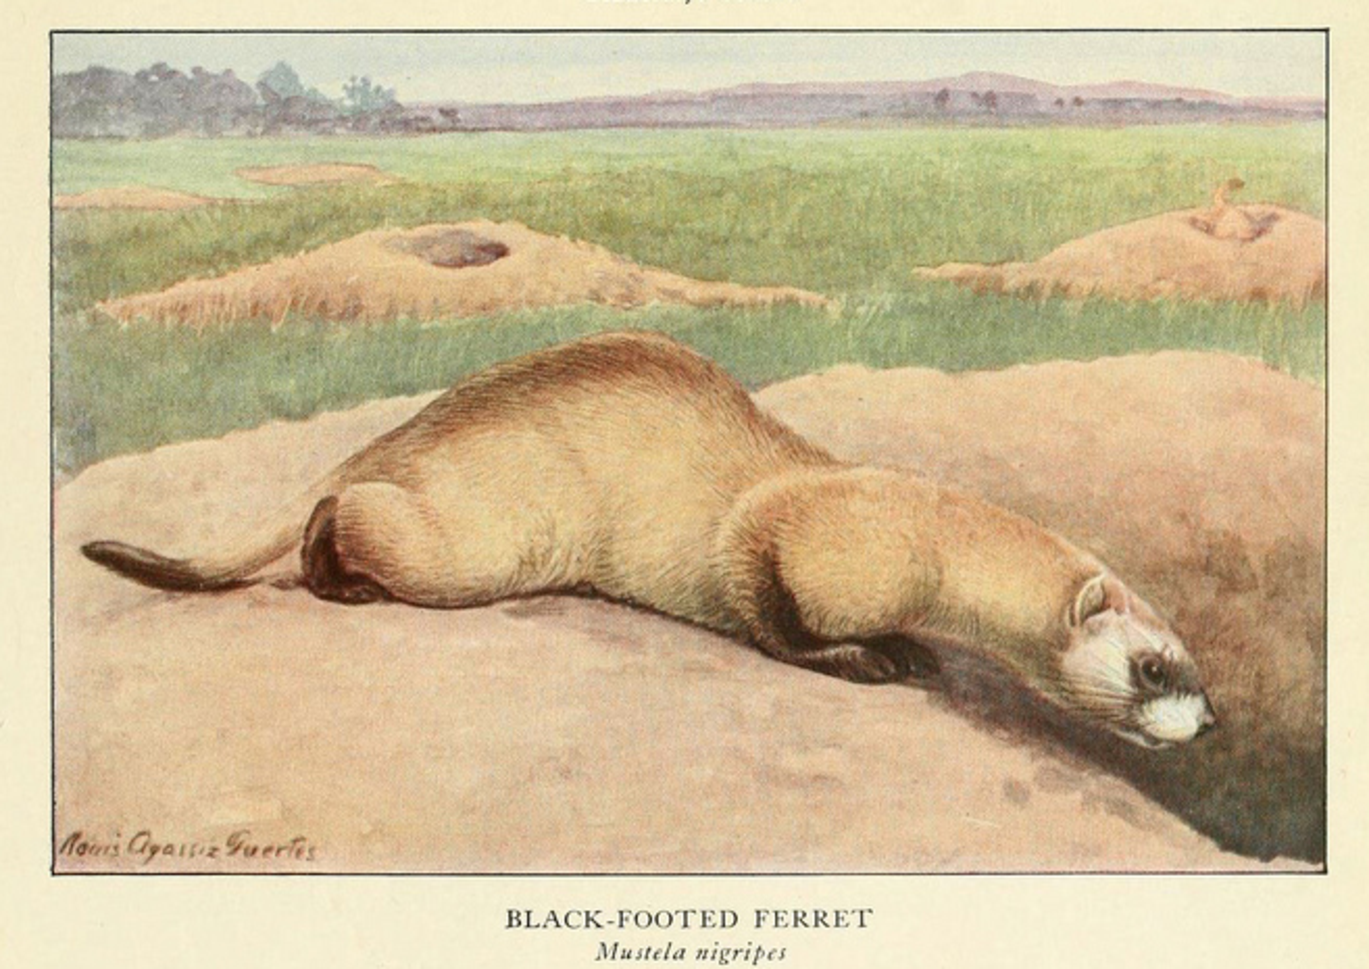
\includegraphics[width=\textwidth]{illustration_images/Genetic_drift/Black_footed_ferrets/Black_footed_ferret.pdf}
\end{center}
\caption{The black-footed ferret ({\it M. nigripes}). \BHLNC{Wild animals of North America, The National geographical
  society, 1918.}{https://www.biodiversitylibrary.org/page/9727900\#page/179/mode/1up}{American Museum of Natural History Library}} \label{fig:black_footed_ferret}
\end{marginfigure}

\begin{figure}
\begin{center}
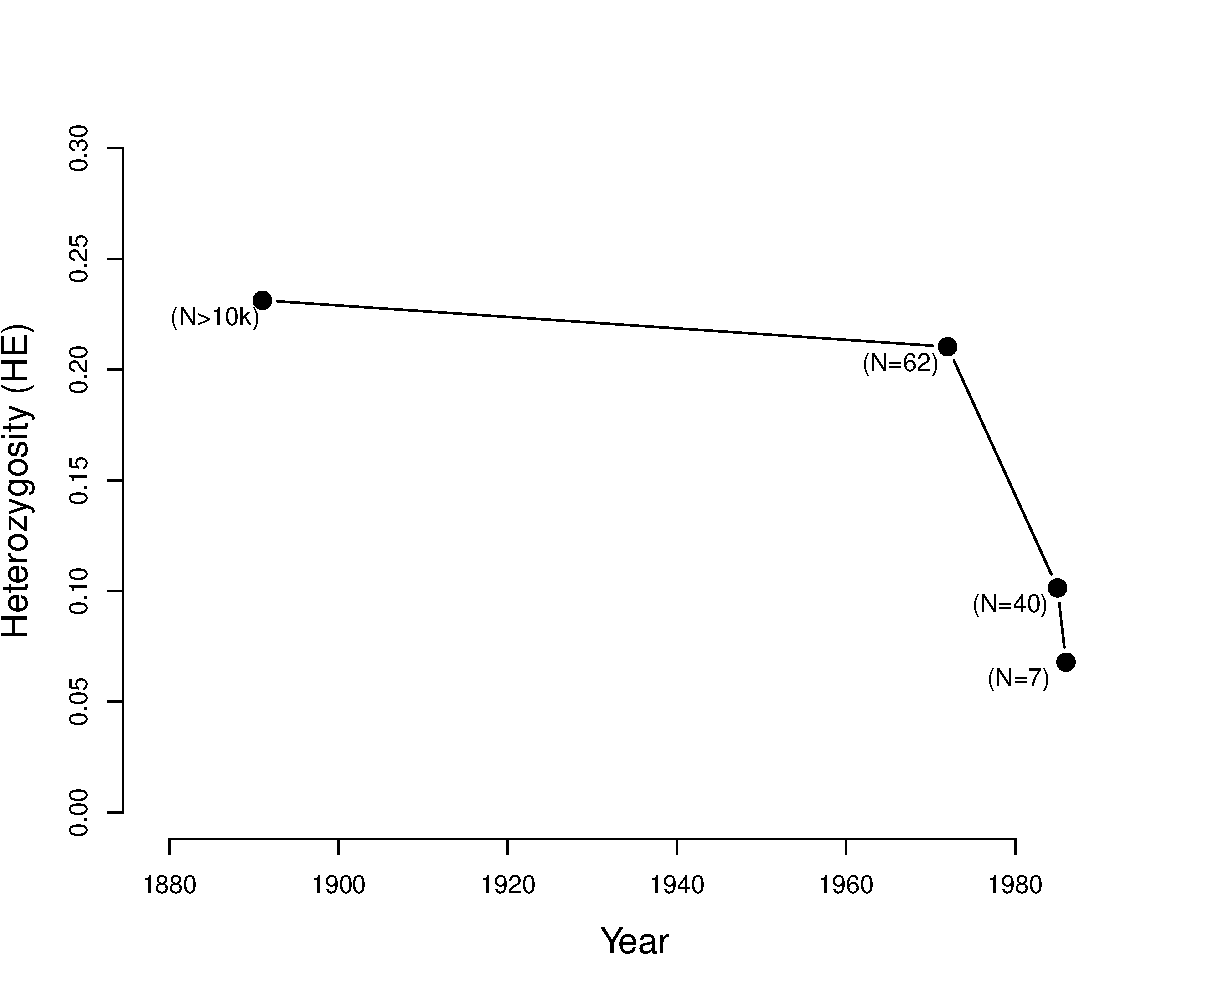
\includegraphics[width= \textwidth]{Journal_figs/genetic_drift/black_footed_ferrets/black_footed_ferrets_He.pdf}
\end{center}
\caption{Loss of heterozygosity in the Black-footed Ferrets in their declining population. Numbers in brackets give estimated number of individuals alive at that time. Data from \citet{Wisely:02}. \gitcode{https://github.com/cooplab/popgen-notes/blob/master/Journal_figs/genetic_drift/black_footed_ferrets/black-footed-ferrets_He.R}} \label{fig:LossHet_ferrets}
\end{figure}

To see how a decline in population size can affect levels of
heterozygosity, let's consider the case of black-footed ferrets ({\it Mustela nigripes}). The black-footed ferret population has declined dramatically through the twentieth century due
to destruction of their habitat.  In 1979, when the last known black-footed ferret died in captivity, they were thought to be
extinct. In 1981, a very small wild population was rediscovered ($40$ individuals), but in 1985 this population
suffered a number of disease outbreaks. All of the $18$ remaining wild individuals
were brought into captivity, 7 of which
reproduced. Thanks to intense captive breeding efforts and conservation work, a
wild population of over 300 individuals has been established
since. However, because all of these individuals are descended from
those 7 individuals who survived the bottleneck, diversity levels
remain low.  \citeauthor{Wisely:02} measured heterozygosity at a number
of microsatellites in individuals from museum collections, showing the sharp drop in diversity as population sizes crashed (see Figure \ref{fig:LossHet_ferrets}).

\begin{question} \label{geo_question} In mathematical population genetics, a
  commonly used approximation is $(1-x) \approx e^{-x}$ for $x << 1$ (formally,
  this follows from the Taylor series expansion of $\exp(-x)$, ignoring second
  order and higher terms of $x$).  This approximation is especially useful for approximating a geometric
  decay process by an exponential decay process, e.g. $(1 - x)^t \approx e^{-xt}$. Using your calculator, or R, check how good of an approximation this is compared to the exact expression for two values of x, $x = 0.1$, and $0.01$, across two different values of t, $t=5$ and $t=50$. Briefly comment on your results.

  %Do this by plotting the geometric decay as
 % points, and the exponential decay as a curve, using different colors for each
 % of these three values of x. Note that you should have a discrete timescale for the
 % geometric decay (e.g. using \texttt{t=seq(0, 18)}) and a near continuous scale
 % for the exponential decay (e.g. using \texttt{t=seq(0, 18, length.out=100)}.
%  Print off your graph and hand it in with your homework.
    % max <- 18; x <- seq(0, max); x1 <- seq(0, max, length.out=100); plot(x, (1-0.5)^x, col='purple', pch=19); lines(x1, exp(-0.5*x1), col='purple'); points(x, (1-0.1)^x, pch=19, col='orange'); lines(x1, exp(-0.1*x1), col='orange'); points(x, (1-0.01)^x, pch=19, col='green'); lines(x1, exp(-0.01*x1), col='green') # messy but works
\end{question}

\subsection{Levels of diversity maintained by a balance between
 mutation and drift} \label{DriftMutationBalance}

Next we're going to consider the amount of neutral polymorphism that can be maintained in a population as a balance between genetic drift removing variation and mutation introducing new neutral variation, see Figure \ref{fig:Mut_Sel_balance} for an example. Note in our example, how no single allele is maintained at a stable equilibrium, rather an equilibrium level of polymorphism is maintained by a constantly shifting set of alleles.

\begin{figure} \begin{center} 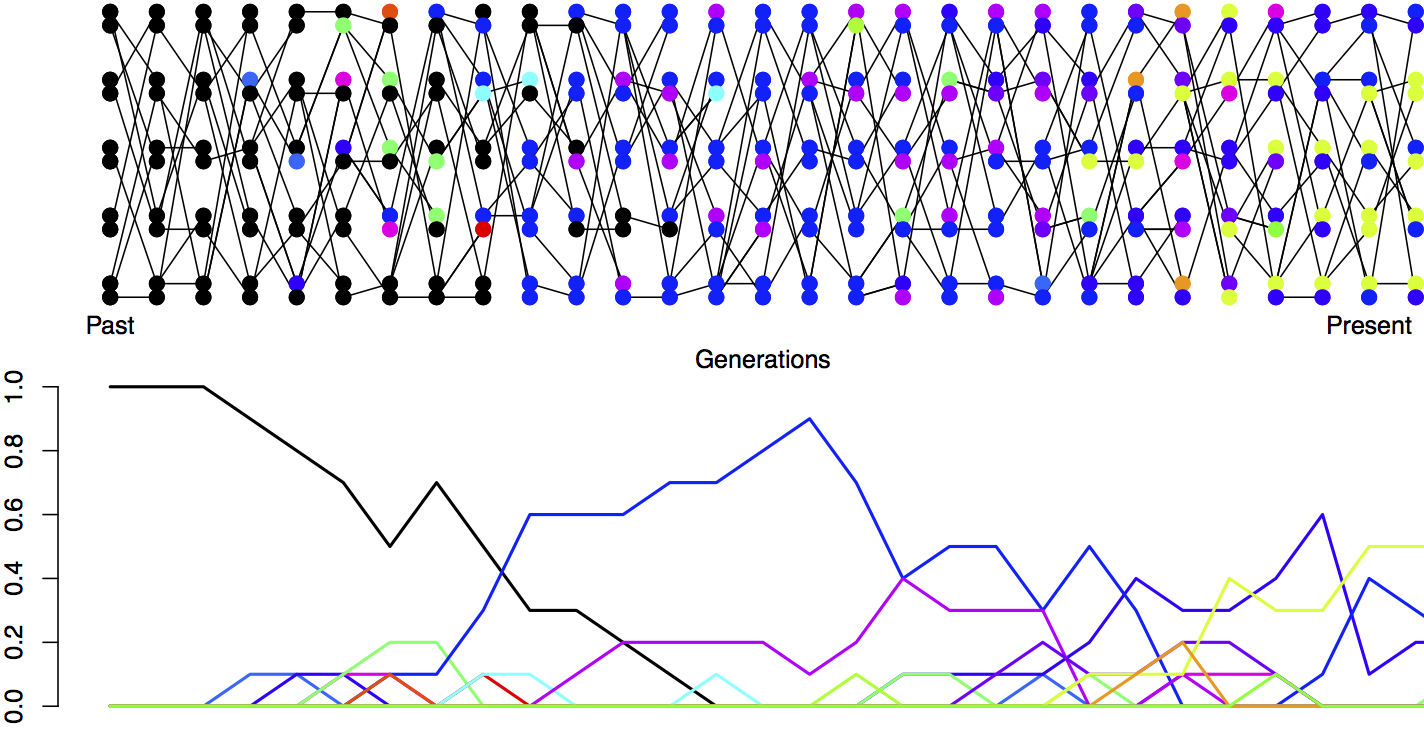
\includegraphics[width= 0.8
\textwidth]{figures/Mut_drift_balance.png} \end{center} \caption{Mutation-drift
balance. A diploid population of 5 individuals. In the first generation
everyone has the same allele (black). Each generation the transmitted allele
can mutate and we generate a new colour. In the bottom plot, I trace the
frequency of alleles in our population over time. The mutation rate we use is very high, simply to maintain diversity in this small population. \gitcode{https://github.com/cooplab/popgen-notes/blob/master/Rcode/Loss_of_heterozyg_varying_pop.R}} \label{fig:Mut_Sel_balance}
\end{figure}

\paragraph{The neutral mutation rate.}
We'll first want to consider the rate at which neutral mutations arise in the population.Thinking back to our discussion of the neutral theory of molecular evolution, let's suppose that there are only two classes of mutation that can arise in our genomic region of interest: neutral mutations and highly deleterious mutations. The total mutation rate at our locus is $\mu$ per generation, i.e. per transmission from parent to child. A fraction $C$ of our mutations are new alleles that are highly deleterious and so quickly removed from the population. We'll call this $C$ parameter the constraint, and it will differ according to the genomic region we consider.  The remaining fraction $(1-C)$ are our neutral mutations, such that our neutral mutation rate is $(1-C)\mu$. This is the per generation rate.
%JRI: modified here to match notation later in chapter where you use $(1-C)\mu$ as the neutral rate

\begin{question}
It's worth taking a minute to get familiar with both how rare, and how common, mutation is. The per base pair mutation rate in humans is around $1.5 \times 10^{-8}$ per generation. That means, on average, we have to monitor a site for $\sim 66.6$ million transmissions from parent to child to see a mutation. Yet populations and genomes are big places, so mutations are common at these levels. \\
{\bf A)} Your autosomal genome is $\sim 3$ billion base pairs long ($3 \times 10^9$). You have two copies, the one you received from your mum and one from your dad. What is the average (i.e. the expected) number of mutations that occurred in the transmission from your mum and your dad to you?\\
{\bf B)} The current human population size is $\sim 7$ billion individuals. How many times, at the level of the entire human population, is a single base-pair mutated in the transmission from one generation to the next?
\end{question}
\paragraph{Levels of heterozygosity maintained as a balance between mutation and selection.}


Looking backwards in time from one generation to the previous generation, we are going to say that two alleles which have the same parental allele (i.e. find their common ancestor) in the preceding generation have \emph{coalesced}, and refer to this
event as a \emph{coalescent event}.

The probability that our pair of randomly sampled alleles have coalesced in the
preceding generation is $\nicefrac{1}{(2N)}$, and the probability that our pair of
alleles fail to coalesce is $1-\nicefrac{1}{(2N)}$.

The probability that a mutation changes the identity of the
transmitted allele is $\mu$ per generation. So the probability of no
mutation occurring is $(1-\mu)$. We'll assume that when a mutation
occurs it creates some new allelic type which is not present in the
population. This assumption (commonly called the infinitely-many-alleles model) makes the math slightly cleaner, and also
is not too bad an assumption biologically. See Figure
\ref{fig:Mut_Sel_balance} for a depiction of mutation-drift balance in
this model over the generations.

This model lets us calculate when our two alleles last shared a common
ancestor and whether these alleles are identical as a result of
failing to mutate since this shared ancestor.  For example, we can work out the probability that our
two randomly sampled alleles coalesce $2$ generations in the past
(i.e. they fail to coalesce in generation $1$ and then coalesce in
generation $2$), and
that they are identical as
\begin{equation}
\left(1- \frac{1}{2N} \right) \frac{1}{2N} (1-\mu)^4
\end{equation}
Note the power of $4$ is because our two alleles have to have failed
to mutate through $2$ meioses each.

More generally, the probability that our alleles coalesce in generation
$t+1$ (counting backwards in time) and are identical due to no mutation to either allele in the
subsequent generations is
%
\begin{equation}
P(\textrm{coal. in t+1 \& no mutations}) =  \frac{1}{2N} \left(1- \frac{1}{2N} \right)^t \left(1-\mu \right)^{2(t+1)}
\end{equation}
%
To make this slightly easier on ourselves let's further assume that $t
\approx t+1$ and so rewrite this as:
\begin{equation}
P(\textrm{coal. in t+1 \& no mutations}) \approx \frac{1}{2N} \left(1- \frac{1}{2N} \right)^t \left(1-\mu \right)^{2t}
\end{equation}
%

This gives us the approximate probability that two alleles will coalesce in the
$(t+1)^\text{th}$ generation. In general, we may not know when two alleles may
coalesce: they could coalesce in generation $t=1, t=2, \ldots $, and so on.
Thus, to calculate the probability that two alleles coalesce in \emph{any}
generation before mutating, we can write:
\begin{align}
  P(\textrm{coal. in any generation \& no mutations}) \approx & P(\textrm{coal. in} \; t=1 \; \textrm{\& no mutations}) \; + \nonumber\\
&  P(\textrm{coal. in} \; t=2 \; \textrm{\& no mutations}) + \ldots \nonumber\\
  %P(\textrm{coal. in} \; t=3 \; \textrm{\& no mutations})  +\ldots \nonumber\\
  = & \sum_{t=1}^\infty P(\textrm{coal. in } \; t \; \textrm{generations \& no mutation})
\end{align}

an example of using the Law of Total Probability, see Appendix eqn \eqref{eqn:law_tot_prob}, combined with the fact that coalescing in a particular generation is mutually exclusive with coalescing in a different generation.

While we could calculate a value for this sum given $N$ and $\mu$, it's
difficult to get a sense of what's going on with such a complicated expression.
Here, we turn to a common approximation in population genetics (and all applied
mathematics), where we assume that $\nicefrac{1}{(2N)} \ll 1$ and $\mu \ll 1$.
This allows us to approximate the geometric decay as an exponential decay (see Appendix eqn \eqref{eqn:Taylor_exp}).
Then, the probability two alleles coalesce in generation $t+1$ and don't mutate
can be written as:
%
\begin{align} P(\textrm{coal. in t+1 \& no mutations}) &\approx \frac{1}{2N}
\left(1- \frac{1}{2N} \right)^t \left(1-\mu \right)^{2t} \\
& \approx \frac{1}{2N} e^{-t/(2N)} e^{-2\mu t } \\
&=\frac{1}{2N} e^{-t(2\mu+1/(2N))} \end{align}
%
Then we can approximate the summation by an integral, giving us:
%

\begin{equation}
\frac{1}{2N} \int_0^{\infty} e^{-t(2\mu+1/(2N))} dt =
\frac{1/(2N)}{1/(2N)+2\mu} = \frac{1}{1+4N\mu}
\end{equation}

The equation above gives us the probability that our two alleles coalesce at some point
in time, and do not mutate before reaching their common
ancestor. Equivalently, this can be thought of as the probability our two
alleles coalesce \emph{before} mutating, i.e. that they are homozygous.

Then, the complementary probability that our pair of alleles are non-identical
(or heterozygous) is simply one minus this. The following equation gives the equilibrium
heterozygosity in a population at equilibrium between mutation and drift:

\marginnote{This result was derived by \citet{kimura1964number} and \citet{malecot:48}  \citep[see][for an English translation, the lack of earlier translation meant this result was missed]{malecot:69}. Technically we're assuming that every new mutation creates a new allele, the so-called "infinitely many alleles" model, otherwise our pair of sequences could be identical due to repeat or back mutation. See this GENETICS \href{http://genestogenomes.org/kimura-crow-infinite-alleles/}{blog post} and \citet{ewens2016motoo} for a nice discussion of the history. }

\begin{equation}
  H = \frac{4N\mu}{1+4N\mu} \label{eqn:hetero}
\end{equation}
 The compound parameter $4N\mu$, the population-scaled mutation rate,
will come up a number of times so we'll give it its own name:
\begin{equation}
\theta = 4N\mu
\end{equation}

So all else being equal, species with larger population sizes should
have proportionally higher levels of neutral polymorphism.

\begin{question}
The sequence-level heterozygosity in {\it Capsella grandiflora} (grand shepherd's purse) is $\sim 2\%$ per base. Assuming a mutation rate of $10^{-9} bp^{-1}$ per generation, what is your estimate of the population size of {\it C. grandiflora}?
\end{question}

\subsection{The effective population size}
\marginnote{the effective population size ($N_e$) is the population size that
would result in the same rate of drift in an idealized population of constant size (following our modeling
assumptions)
as that observed in our true population .}

In practice, populations rarely conform to our assumptions of being constant in size with low variance in reproductive success. Real populations experience dramatic fluctuations in size, and there is
%JRI: perhaps missed, but where did you spell out these assumptions previously?
often high variance in reproductive success. Thus rates of drift in
natural populations are often a lot higher than the census population
size would imply. See Figure \ref{fig:LossHet_varying_pop}  for a depiction of
a repeatedly bottlenecked population losing diversity at a fast rate.

\begin{figure}
\begin{center}
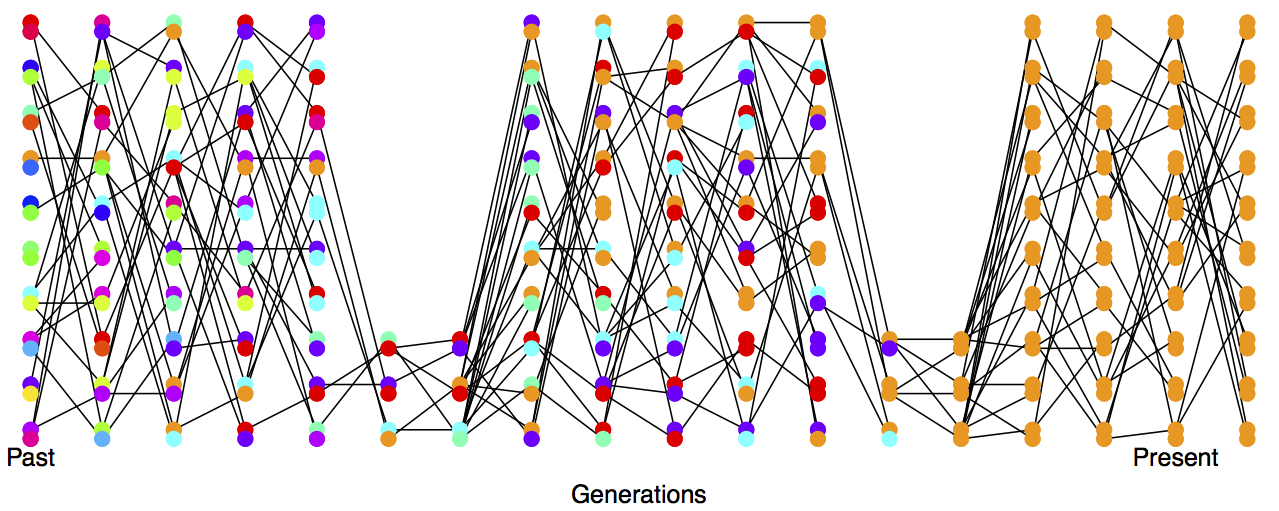
\includegraphics[width= \textwidth]{figures/Loss_of_he_col_alleles_varying_pop_dark.png}
\end{center}
\caption{Loss of heterozygosity over time in a bottlenecking population. A diploid population of 10 individuals, that bottlenecks
  down to three individuals repeatedly. In the first generation, I colour every allele a different
colour so we can track their descendants. There are no new
  mutations. \gitcode{https://github.com/cooplab/popgen-notes/blob/master/Rcode/Loss_of_heterozyg_varying_pop.R}} \label{fig:LossHet_varying_pop}
\end{figure}


To cope with this discrepancy, population geneticists often invoke the concept of
an \emph{effective population size} ($N_e$). In many situations (but not all), departures from model assumptions can be captured by substituting $N_e$ for $N$.
\\


If population sizes vary rapidly in size, we can (if certain conditions are met) replace our population size by the harmonic mean population size.
Consider a diploid population of variable size, whose size is $N_t$ $t$ generations into the
past. The probability our pairs of alleles have not coalesced by generation $t$ is
given by
\begin{equation}
\prod_{i=1}^{t} \left(1-\frac{1}{2N_i} \right) \label{eqn:var_pop_coal}
\end{equation}
Note that this simply collapses to our original expression
$\left(1-\frac{1}{2N } \right)^t $ if $N_i$ is constant. Under this model, the rate of loss of heterozygosity in this population is equivalent to
a population of effective size
\begin{equation}
N_e =\frac{1}{\frac{1}{t} \sum_{i=1}^{t} \frac{1}{N_i} }. \label{eq:Ne_harmonic}
\end{equation}
This is the harmonic mean of the varying population size. \sidenote[][-6cm]{
To see this, note that if $1/(N_i)$ is
small, then we can approximate \eqref{eqn:var_pop_coal} using the exponential approximation:
\begin{equation}
\prod_{i=1}^{t} \exp \left( -\frac{1}{2N_i} \right)   =
\exp \left(- \sum_{i=1}^{t} \frac{1}{2N_i} \right) .
\end{equation}
When we put the product inside the exponent, it becomes a sum.  We can also write the probability of not coalescing by generation $t$ in a population of constant size ($N_e$) as an exponential, so that it takes the same form as the expression above on the right. Comparing the exponent in the two cases, we see
\begin{equation}
\frac{t}{2N_e} = \sum_{i=1}^{t} \nicefrac{1}{(2N_i)}
\end{equation}
So that if we want a constant effective population size ($N_e$) that has the same
rate of loss of heterozygosity as our variable population, we need to rearrange and solve this equation to give \eqref{eq:Ne_harmonic}. }


Thus our effective population size, the size of an idealized constant
population which matches the rate of genetic drift, is the harmonic
mean true population size over time. The harmonic mean is very
strongly affected by small values, such that if our population size is
one million $99\%$ of the time but drops to $1000$ every hundred or
so generations, $N_e$ will be much closer to $1000$ than a
million. \\


%would result in the same rate of drift
%Luckily, in many (not all) situations, departures from model assumptions can be captured by substituting Ne for N, i.e., by plugging in a fictitious N that leads to the same level of genetic drift as observed.

\begin{figure}
\begin{center}
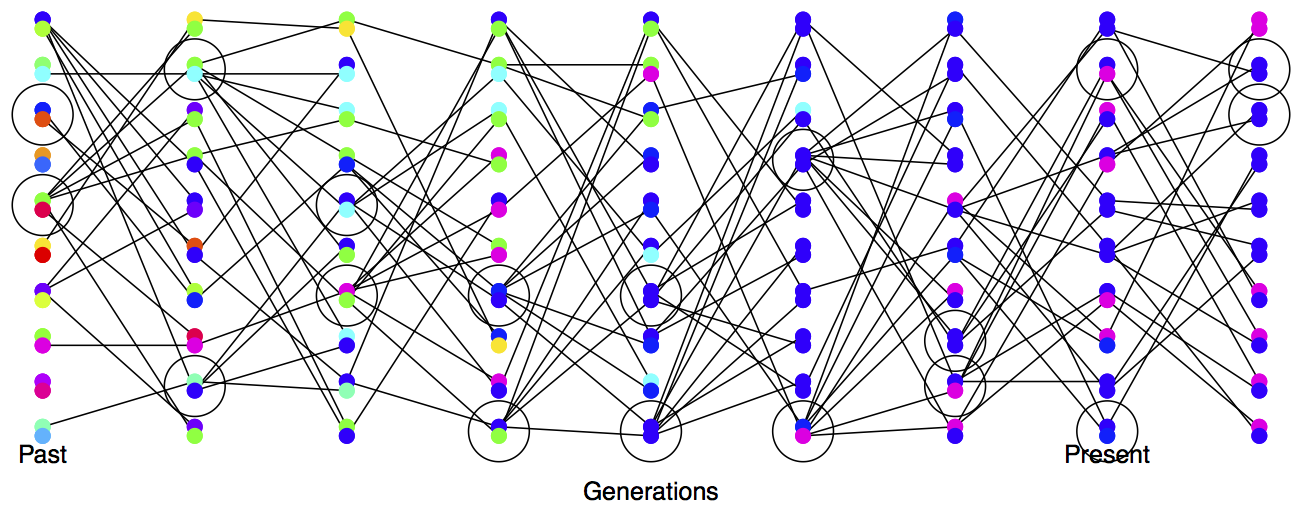
\includegraphics[width= \textwidth]{figures/Loss_of_he_col_alleles_varying_RS.png}
\end{center}
\caption{High variance on reproductive success increases the rate of genetic drift. A diploid population of 10 individuals, where the circled
  individuals have much higher reproductive success. In the first generation I colour every allele a different
colour so we can track their descendants, there are no new
  mutations. \gitcode{https://github.com/cooplab/popgen-notes/blob/master/Rcode/Loss_of_heterozyg_varying_pop.R}} \label{fig:LossHet_varying_RS}
\end{figure}

Variance in reproductive success will also affect our effective
population size. Even if our population has a large constant size $N$
individuals, if only small proportion of them get to reproduce, then
the rate of drift will reflect this much smaller number of reproducing
individuals. See Figure \ref{fig:LossHet_varying_RS} for a depiction of the higher rate of drift
in a population where there is high variance in reproductive success.

To see one example of this, consider the case where $N_F$ of  females get to reproduce and $N_M$ males get reproduce.
While every individual has a mother an a father, not every individual gets to be a parent. In practice, in many animal species far more females get to reproduce than males, i.e. $N_M <N_F$, as a few males get many mating opportunities and many males get no/few mating opportunities \citep[see ][for a broad analysis, and note that there a certainly many exceptions to this general pattern]{janicke:16}. When our two alleles pick an ancestor, $25\%$ of the time our alleles were both in a female ancestor, in which case they are IBD with probability $1/(2N_F)$, and $25\%$ of the time they are both in a
male ancestor, in which case they coalesce with probability
$1/(2N_M)$.
%JRI: this felt like it came out of nowhere. ``when our two alleles''  -- which two? from some example? ``$25\%$ of the time our alleles were both in a female ancestor'' -- this sould be explained. are you assuming 50% females and 50% males?
The remaining $50\%$ of the time, our alleles trace back to two individuals of different sexes in the prior generation and so cannot coalesce.  Therefore, our probability of coalescence in the preceding generation is
\begin{equation}
\frac{1}{4}\left(\frac{1}{2N_M} \right)+\frac{1}{4}\left(\frac{1}{2N_F} \right) %=
%\frac{1}{8}\frac{N_F+N_M}{N_FN_M}
\end{equation}
i.e. the rate of coalescence is the harmonic mean of the two sexes' population sizes, equating this to $\frac{1}{2N_e}$ we find

\begin{marginfigure}
\begin{center}
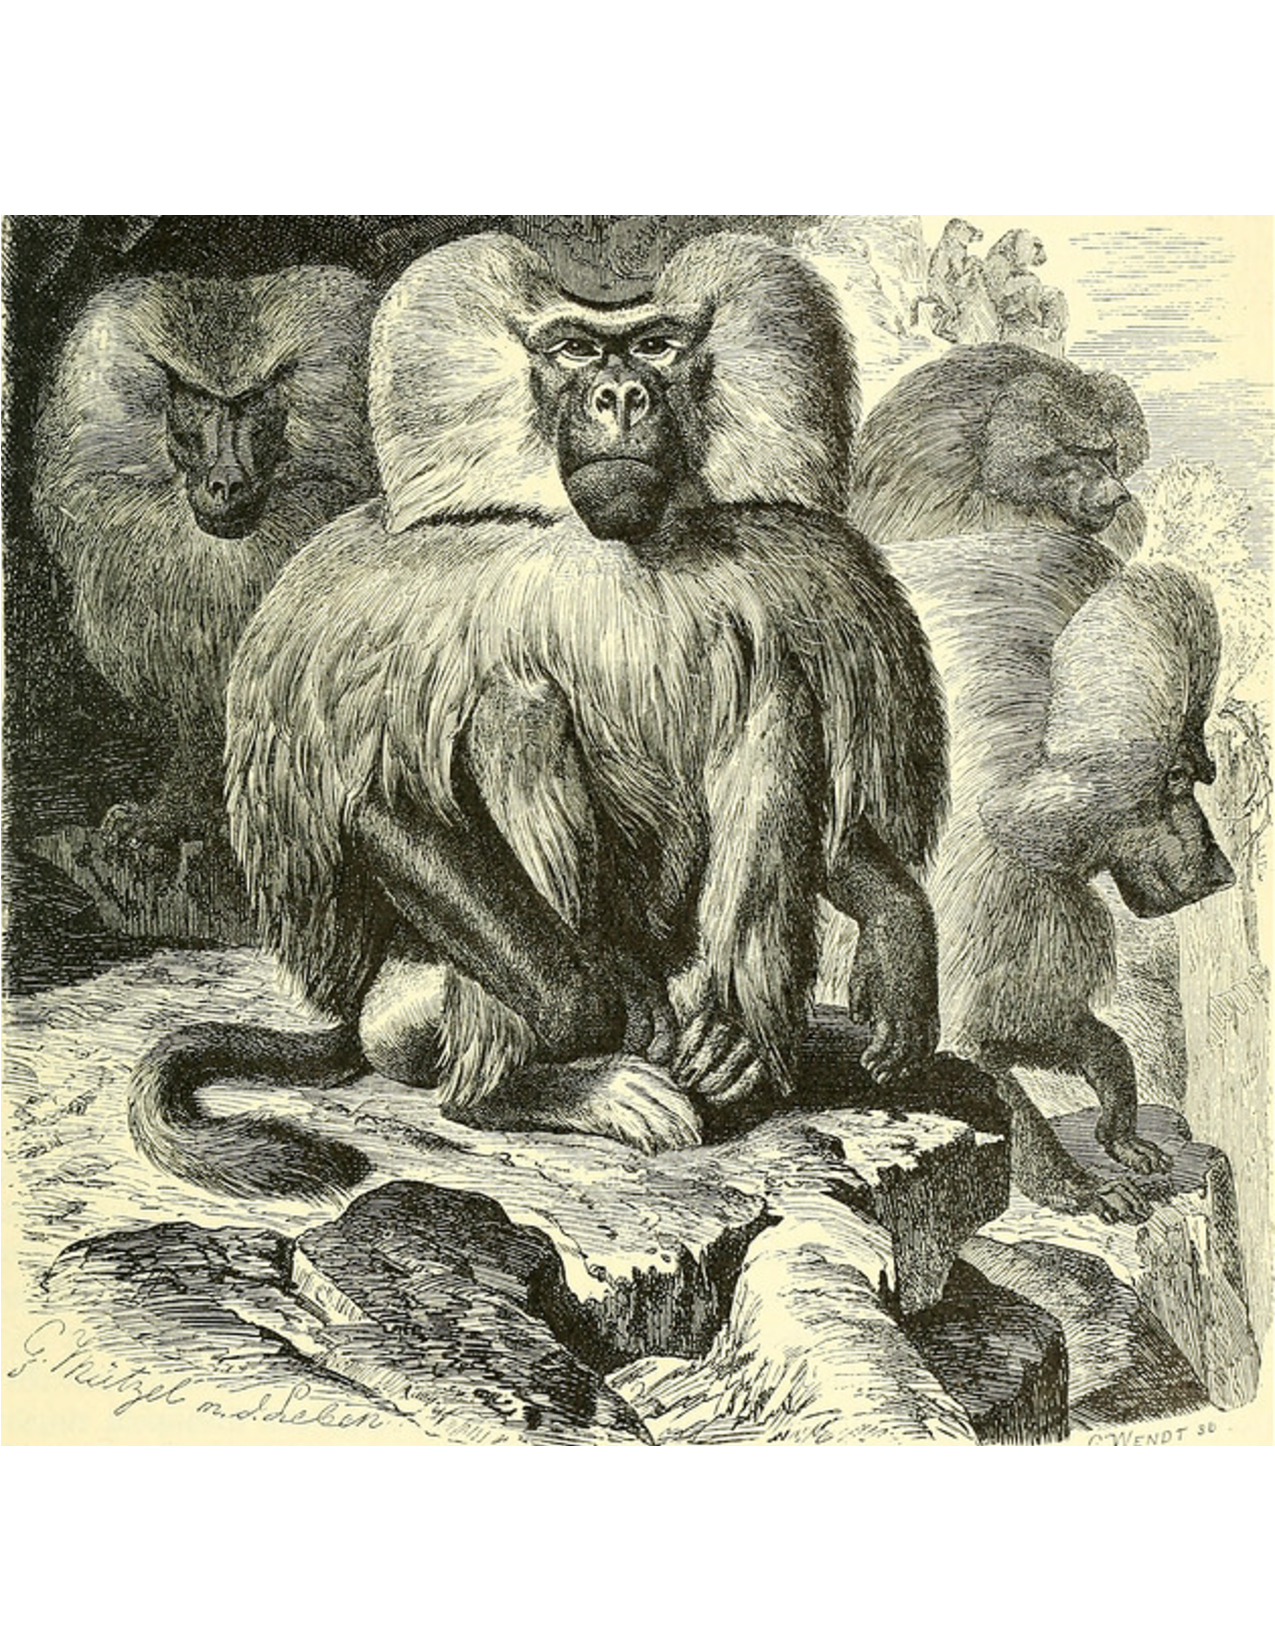
\includegraphics[width= 0.7 \textwidth]{illustration_images/Genetic_drift/Hamadryas_baboon/Hamadryas_baboon.pdf}
\end{center}
\caption{Male Hamadryas baboons. Up to ten females live in a harem with a single male.\BHLNC{Brehm's Tierleben (Brehm's animal life). Brehm,
  A.E. 1893.}{https://archive.org/stream/brehmstierlebena001breh/\#page/181/mode/1up}{University of Illinois Urbana-Champaign}  %Brehm's animal life
} \label{fig:Hamadryas_baboon}
\end{marginfigure}

\begin{equation}
N_e = \frac{4N_FN_M}{N_F+N_M}
\end{equation}
Thus if reproductive success is very skewed in one sex (e.g. $N_M \ll
N/2$), our effective population size will be much reduced as a result. For more on how different evolutionary forces affect the rate of genetic drift, and their impact on the effective population size, see \citet{charlesworth:09}.\\

\begin{question}
You are studying a population of 500 male and 500 female Hamadryas baboons. Assume that all of the females but only 1/10 of the males get to mate:
{\bf A)} What is the effective population size for the autosome?\\
{\bf B)} Do you expect the {\it ratio} of X-chromosome to autosomal diversity to be higher or lower in this species compared to a species where the sexes have more similar variance in reproductive success? Explain the intuition behind your answer.
 \end{question}

\graham{Add X chromosome Ne?}
\section{The Coalescent and patterns of neutral diversity}

\begin{quote}
``Life can only be understood backwards; but it must be lived
forwards'' -- Kierkegaard
\end{quote}

\paragraph{Pairwise Coalescent time distribution and the number of
 pairwise differences.}
Thinking back to our calculations we made about the loss of neutral heterozygosity
and equilibrium levels of diversity (in Sections \ref{LossofHet} and \ref{DriftMutationBalance}), you'll note that we could first specify
which generation a pair of sequences coalesce in, and then calculate
some properties of heterozygosity based on that. That's because neutral
mutations do not affect the probability that an individual transmits
an allele, and so don't affect the way in which we can trace ancestral lineages
back through the generations. \\
\marginnote{In discussing the coalescent we'll be making use of random variables, e.g. number of generations back to the common
ancestor of a pair of sequences is a random variable. We'll also use the expectation of random variables, e.g. the average number of generations back to the common
ancestor of a pair of sequences. Have a look at sections \ref{Section_rv} and \ref{appendix:expectation}.}

As such, it will often be helpful to consider the time to the common
ancestor of a pair of sequences, and then think of the impact of that time to coalescence
on patterns of diversity. See Figure \ref{fig:Coalescent_simulation}
for an example of this.

\begin{figure}
\begin{center}
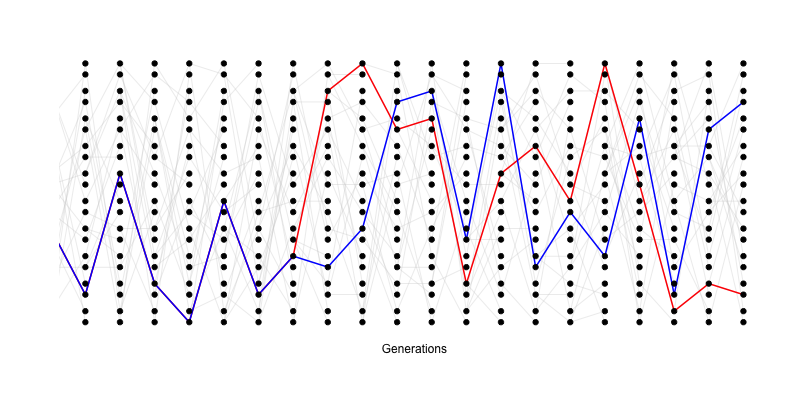
\includegraphics[width=\textwidth]{figures/Coalescent.png}
\end{center}
\caption[][3cm]{A simple demonstration of the coalescent process. The simulation
  consists of a diploid population of 10 individuals (20 alleles). In
  each generation, each individual is equally likely to be the parent
  of an offspring (and the allele transmitted is indicated by a light
  grey line).  We track a
  pair of alleles, chosen in the present day, back 14 generations
  until they find a common ancestor. \gitcode{https://github.com/cooplab/popgen-notes/blob/master/Rcode/track_alleles.R} } \label{fig:Coalescent_simulation}  %https://github.com/cooplab/popgen-notes/blob/master/Rcode/track_alleles.R
\end{figure}

The probability that a pair of alleles
have failed to coalesce in $t$ generations and then coalesce in the
$t+1$ generation back is
\begin{equation}
 P(T_2=t+1) = \frac{1}{2N} \left(1- \frac{1}{2N} \right)^{t} \label{eqn:coal_time_dist}
\end{equation}
For example, the probability that a pair of sequences coalesce three generations back is the probability that they fail to coalesce in generation 1 and 2, which is $ \left(1- \nicefrac{1}{2N} \right) \times \left(1- \nicefrac{1}{2N} \right)$, multipled by the probability that they find a common ancestor, i.e. coalesce, in the third generation, which happens with probability $\nicefrac{1}{2N}$. 

From the form of eqn \eqref{eqn:coal_time_dist} we can see that the coalescent time of our pair of alleles is a Geometrically distributed random variable,\sidenote{See Appendix eqn \eqref{eqn:geometric_def} and surrounding text for more on the Geometric distribution.} where the probability of success is $p=\nicefrac{1}{2N}$. The waiting time for a pair of lineages to coalesce is like the number of tails thrown while waiting for a head on a coin with the probability of a head is $\nicefrac{1}{2N}$, i.e. id the population is large we might be waiting for a long time for our pair to coalesce. We'll denote this geometric distribution by $T_2 \sim  \text{Geo}(1/(2N))$. 
%JRI: not clear you're consistent with capitalization of prob. distributions.
The expected (i.e. the mean over many replicates) coalescent time of a pair of alleles is then
\begin{equation}
\E(T_2) = 2N
\end{equation}
generations. This form to the expectation follows from the fact that the mean of an geometric random variable is $\nicefrac{1}{p}$.\\


Conditional on a pair of alleles coalescing $t$ generations ago,
there are $2t$ generations in which a mutation could occur. See Figure \ref{fig:pair_coal_muts} for an example. If the per
generation mutation rate is $\mu$, then the expected number of
mutations between a pair of alleles coalescing $t$ generations ago is
$2 t\mu$ (the alleles have gone through a total of $2t$ meioses since they last shared a common ancestor).
\begin{marginfigure}
\begin{center}
  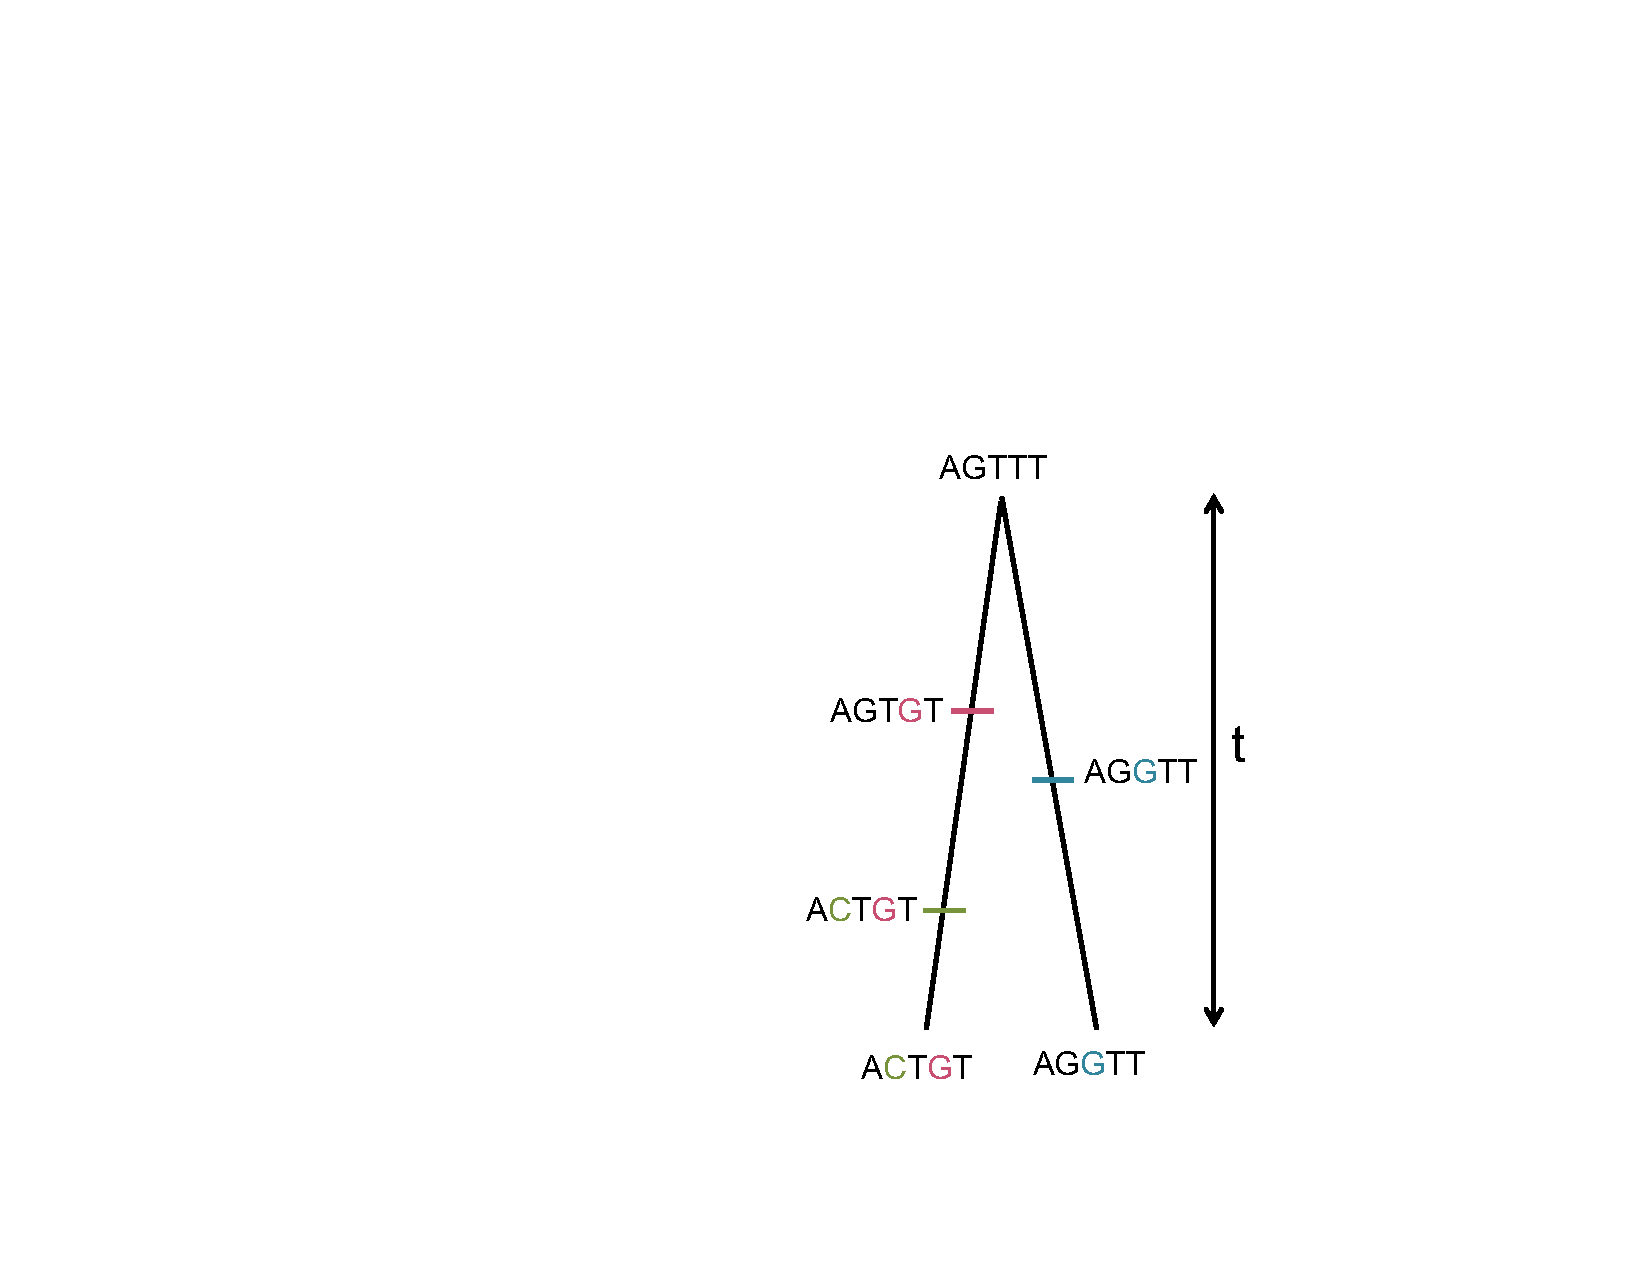
\includegraphics[width =
  \textwidth]{figures/Coalescent/Coal_two_lineages_muts.pdf}  \end{center}
\caption{The ancestral lineages of a pair of sequences coalese $t$ generations in the past. There are $2t$ generations that mutations could occur in that would be differences between our sequences. Three mutations have occured in this time changing the ancestral sequence (AGTTT) to the sequences at the bottom of the picture. } \label{fig:pair_coal_muts}
\end{marginfigure}
So we can write the expected
number of mutations ($S_2$) separating two alleles drawn at random from the
population as %\erin{I added subscript 2 to all the T's, which I think is appropriate}
\begin{align}
\E(S_2) &= \sum_{t=0}^{\infty} \E(S_2 | T_2=t) P(T_2=t) \nonumber\\
& =\sum_{t=0}^{\infty} 2 \mu t P(T_2=t) \nonumber\\
& =2\mu \E(T_2)  \nonumber\\
& = 4 \mu N
\end{align}
this makes use of the law of total expectation (see Appendix eqn \eqref{eqn:tot_exptation_def}) to average which generation our pair of sequences coalesce in. 
%As our expected coalescent time is $2N$ generations (which follows from the expected value of exponential distributions), the expected
%number of mutations separating two alleles drawn at random from the
%population is
%
%\begin{align}
 % \E(j) &= 2\mu\E(t) \\ \nonumber
 % &= 4N\mu \\
 % &= \theta \nonumber
%\end{align}
We'll assume that mutation is rare enough that it never happens at the same basepair twice, i.e. no multiple hits, such that we get to see all of the mutation events that separate our pair
of sequences. This is assumption that repeat mutation is vanishingly rare at a basepair is called the {\emph infinitely-many-sites} assumption,
which should hold if $N\mu_{BP} \ll 1$, where $\mu_{BP}$ is the mutation rate per base pair. Thus the number of
mutations between a pair of sites is the observed number of
differences between a pair of sequences. In the previous chapter we denote the observed number of pairwise differences at putatively neutral
sites separating a pair of sequences as $\pi$ (we usually average this over a
number of pairs of sequences for a region). Therefore, under our simple, neutral, constant population-size model we expect
\begin{equation}
\E(\pi) = 4 N \mu = \theta
\end{equation}
So we can get an empirical estimate of $\theta$ from
$\pi$, let's call this $\widehat{\theta}_{\pi}$, by setting $\widehat{\theta}_{\pi}=\pi$., i.e. our observed level of pairwise genetic diversity.  If we
have an independent estimate of $\mu$, then from setting $\pi =\widehat{\theta}_{\pi} = 4N\mu$ we can furthermore obtain an estimate of the population
size $N$ that is consistent with our levels of neutral polymorphism. If we estimate the population size this way, we should call it the effective coalescent population size ($N_e$). It's best to think about $N_{e}$ estimated from neutral diversity as a long-term effective population size for the species, but there are many caveats that come along with that assumption. For example, past bottlenecks and population expansions are all subsumed into a single number and so this estimated $N_{e}$ may not be very representative of the population size at any time. That said, it's not a bad place to start when thinking about the rate of genetic drift for neutral diversity in our population over long time-periods. \sidenote[][]{Up to this point we've been describing only neutral processes, however, selection can also alter levels of polymorphism. For example, if some synonymous sites directly experience selection, then even if we use $\pi$ calculated for synonymous changes we may underestimate the coalescent effective population size. As we'll see later in the notes, selection at linked sites can also impact neutral diversity. As such, if we can, we may want to use genomic sites subject to the weakest selective constraints, and also far from gene-dense or otherwise very constrained regions of the genome, to estimate $N_e$ from $\pi$. But even then caution is warranted. }

Lets take a moment to distinguish our expected heterozygosity (eqn. \ref{eqn:hetero}) from our expected number of pairwise differences ($\pi$). Our expected heterozygosity is the probability that two alleles at a locus, sampled from a population at random, are different from each other. If one or more mutations have occurred since a pair of alleles last shared a common ancestor, then our sequences will be different from each other. On the other hand, our $\pi$ measure keeps track of the average total number of differences between our loci. As such, $\pi$ is often a more useful measure, as it records the number of differences between the sequences, not just whether they are different from each other (however, for certain types of loci, e.g. microsatellites, heterozygosity is often used as we cannot usually count up the minimum number of mutations in a sensible way). In the case where our locus is a single basepair, the two measures will usually be close to one another, as $H \approx \theta$ for small values of $\theta$. For example, comparing two sequences at random in humans, $\pi \approx 1/1000$ per basepair, and the probability that a specific base pair differs between two sequences is $\approx 1/1000$. However, these two quantities start to differ from each other when we consider regions with higher mutation rates. For example, if we consider a 10kb region, our mutation rate will 10,000 times larger than a single base pair. For this length of sequence the probability that two randomly chosen haplotypes differ is quite different from the number of mutational differences  between them. (Try a mutation rate of $10^{-8}$ per base and a population size of $10,000$ in our calculations of $\E[\pi]$ and H to see this.)

%\erin{can you give an intuitive example when per bp $\pi$ is very different from heterozygosity? Or is this distinction really just key when we're talking about larger loci?}

\begin{marginfigure}
\begin{center}
  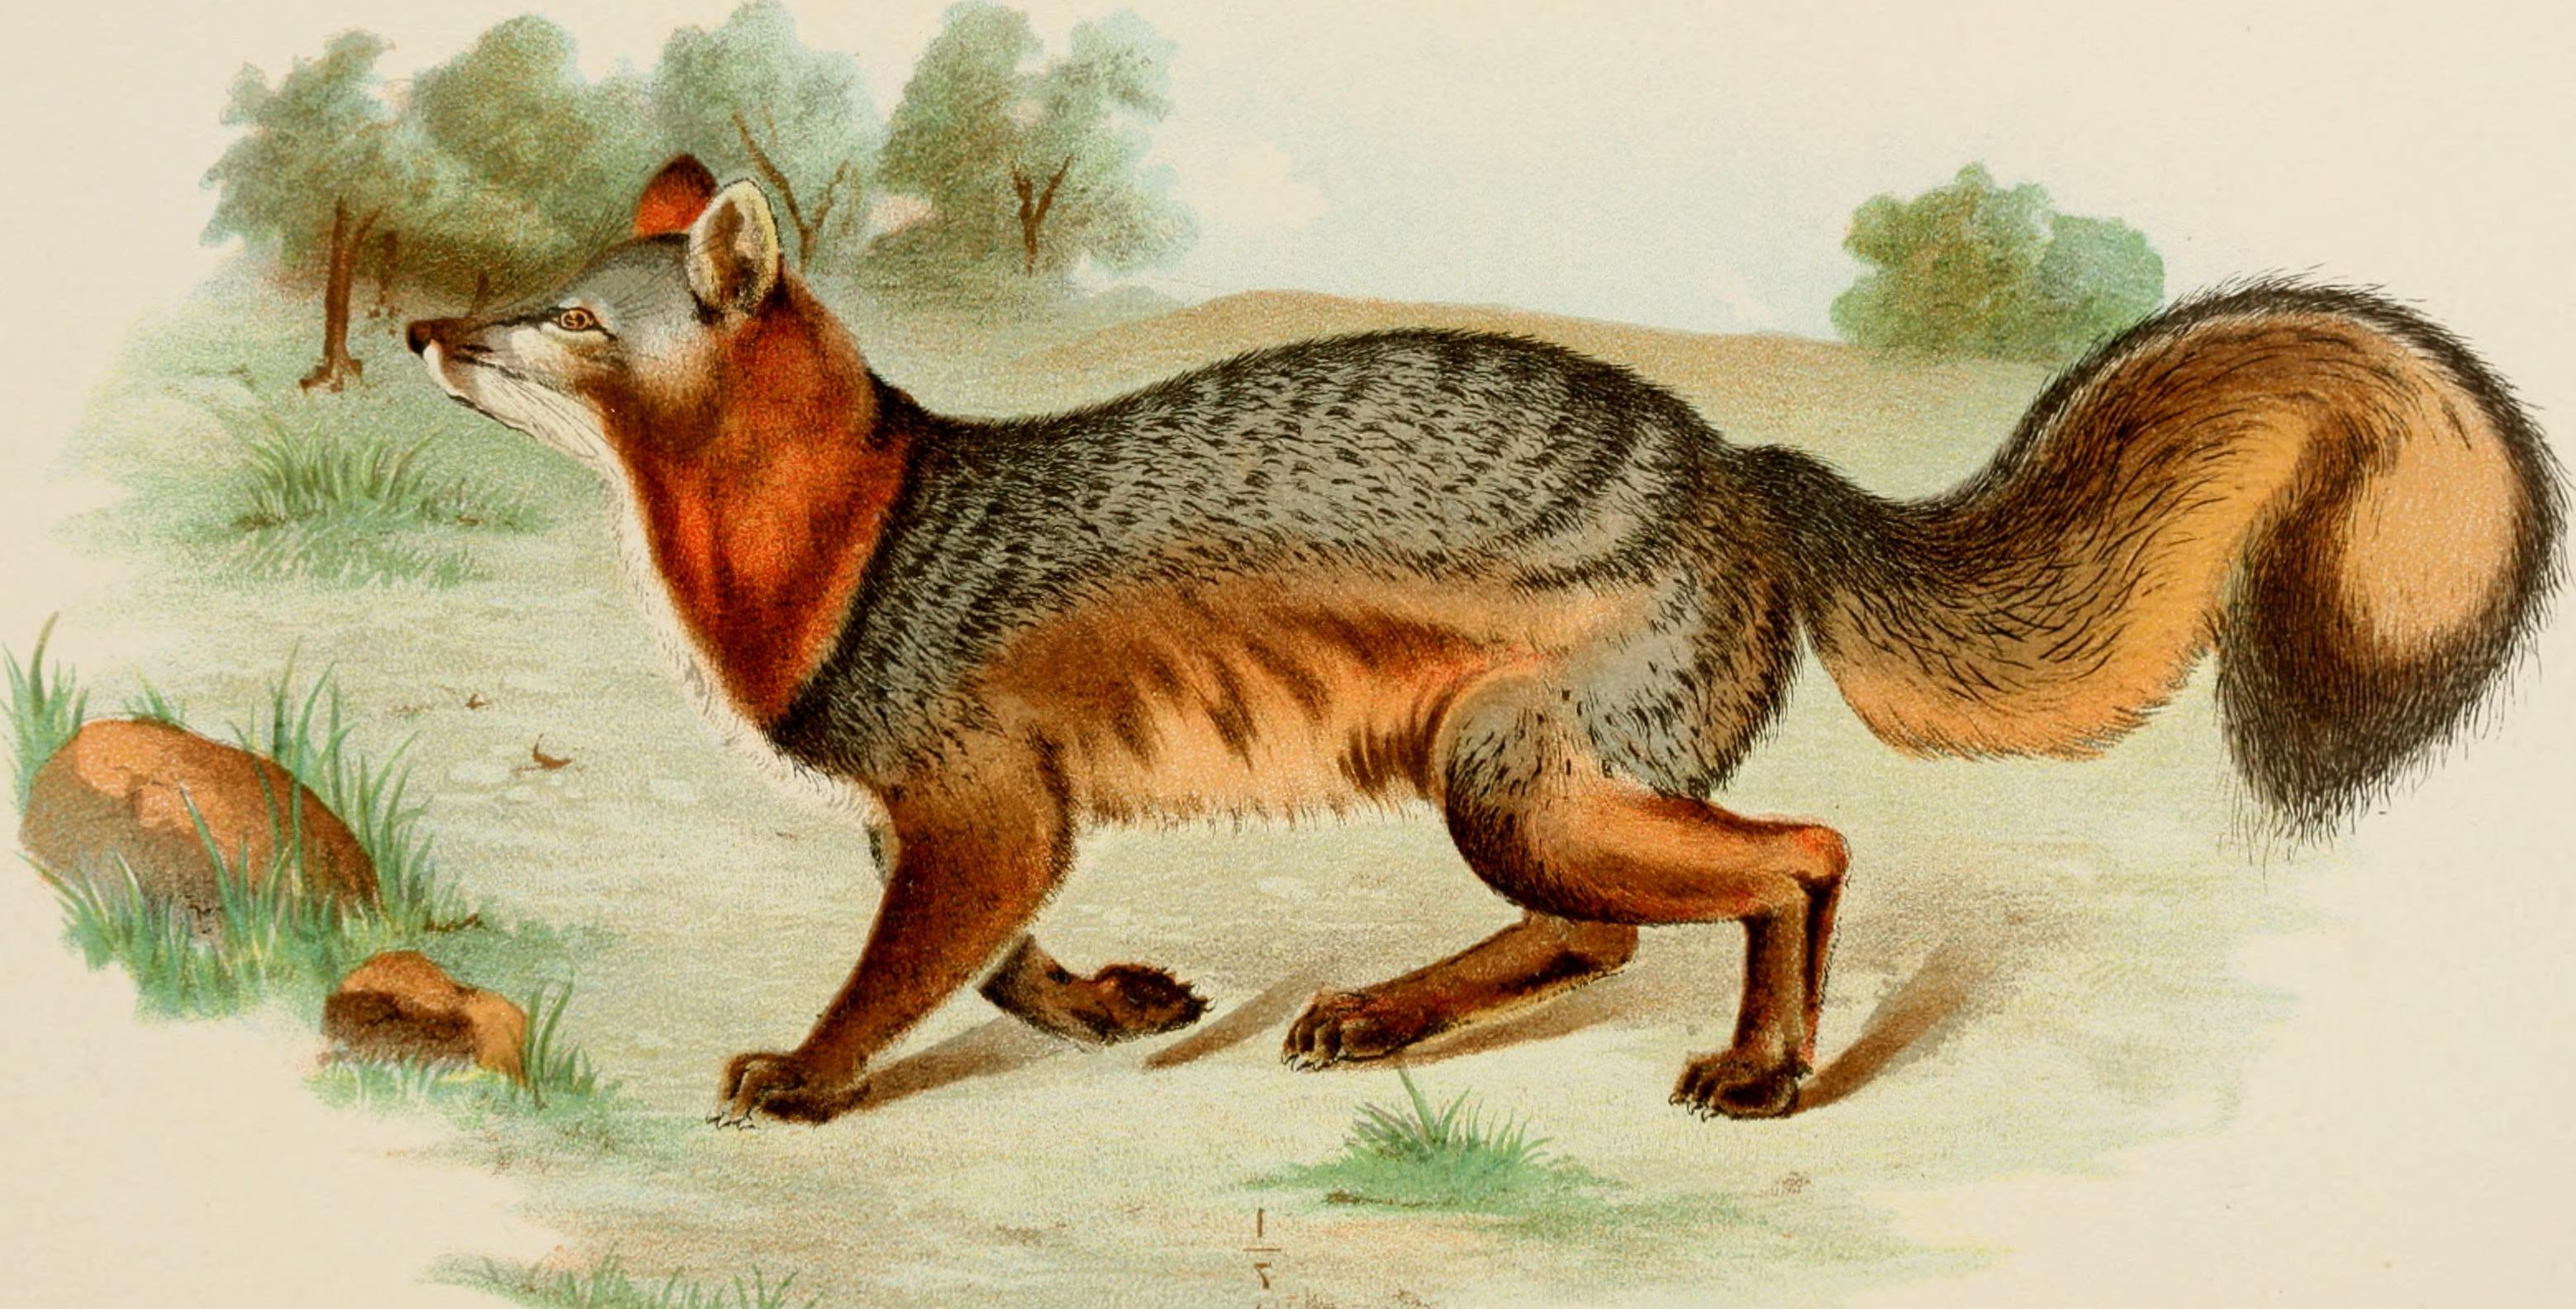
\includegraphics[width =
  \textwidth]{illustration_images/Quant_gen/Grey_fox/14770789583_4db7ec5164_o.jpg}  %https://www.flickr.com/photos/internetarchivebookimages/14770789583/in/photolist-axdicF-ovfa8V-odM3sY-bCrnQ8-ovgYXn-tiQfMQ-odMpu5-x1xCJu-wQ7qT7-wE7kfs-xEZQd1-wK4YSh-ovWx4g-wpDZzF-xjvQ89-tHDjuS-w9Wit5-xEvyhH-xjCbKD-u4q3Qe
\end{center}
\caption{Gray Fox, {\it Urocyon cinereoargenteiis}. \BHLNC{Diseases and enemies of poultry. Pearson and Warren. (1897)}{https://archive.org/stream/diseasesenemieso00pearrich/diseasesenemieso00pearrich\#page/n663/mode/1up}{University of California Libraries}}
\end{marginfigure}


\begin{question}
\citet{robinson:16} found that the endangered Californian Channel Island fox on San Nicolas had very
low levels of diversity ($\pi =0.000014 \text{bp}^{-1}$) compared to
its close relative the California mainland gray fox ($0.0012\text{bp}^{-1}$). \\
%\bf A How many sites do you expect to differ between two samples
%sequenced over a 100kb region in each of these populations?\\
{\bf A)} Assuming a mutation rate of $2\times 10^{-8}$ per bp, what
effective population sizes do you estimate for these two populations?
\\
{\bf B)} Why is the effective population size of the Channel Island fox
so low? [Hint: quickly google Channel island foxes to read up on their
history, also to see how ridiculously cute they are.]
\end{question}


\begin{question}
In your own words describe why the coalescent time of a pair of lineages scales linearly with the (effective) population size.
%The long-term $N_e$ estimated from genetic diversity within most human populations is roughly $10,000$, and the generation time of humans is $\sim$30 years. What is the average time, in years, that we have to go back to to find the most recent common ancestor for  a pair of sequences drawn from the same human population?
\end{question}


\paragraph{More details on the pairwise coalescent and the randomness of mutation.}
We found that our pairwise coalescent times followed a Geometric distribution, eqn  \eqref{eqn:coal_time_dist}. However, that assumes discrete generations and we'll often was to think about populations that lack discrete generations (i.e. individuals reproducing at random times with some mean generation time). Using our exponential approximation, we can see  that is
\begin{equation}
\approx \frac{1}{2N} e^{-t/(2N)}
\end{equation}
and so think of  a continuous random variable, i.e. we could say that the coalescent time of a pair of sequences ($T_2$) is approximately exponentially distributed with a rate $1/(2N)$, i.e. $T_2 \sim \text{Exp}\left( 1/(2N) \right)$. Formally we can do this by taking the limit of the discrete process more carefully. See Appendix eqn \eqref{eqn:exp_rv_def} for more on exponential random variables. 

We've derived the expected number of differences between a pair of sequences and talked about how variable the coalescent time is for a pair of sequences. The mutation process is also very variable; even if two sequences coalesce in the very distant past by chance, they may still be identical in the present if there was no mutation during that time.

Conditional on the coalescent time $t$, the probability that our pair of alleles are separated by $S_2$ mutations since they last shared a common ancestor is bionomially distributed
\begin{equation}
P(S_2 | T_2 = t ) = {2t \choose j} \mu^{j} (1-\mu)^{2t-j}
\end{equation}
i.e. mutations happen in $j$ generations and do not happen in $2t-j$
generations (with ${2t \choose j}$ ways this combination of events can possibly
happen). See Appendix eqn \eqref{eqn:binomial_dist} for discussion of the binomial distribution. Assuming that $\mu \ll 1$ and that $2t-j \approx 2t$, then we
can approximate the probability that we have $S_2$ mutations as a
Poisson distribution:
\begin{equation}
P(S_2 | T_2 = t ) = \frac{ (2 \mu t )^{j} e^{-2\mu t}}{j!}
\end{equation}
i.e. a Poisson with mean $2\mu t $. This is an example of taking the binomial distribution to its Poisson distribution limit, see Appendix eqn \eqref{eqn:bionom_to_poiss} for more details. We'll not make much use of this result, but it is very useful in thinking about how to simulate the process of mutation.\\

\section{The coalescent process of a sample of alleles.}

Usually we are not just interested in pairs of alleles, or the
average pairwise diversity. Generally we are interested in the properties of
diversity in samples of a number of alleles drawn from the population.
Instead of just following a pair of lineages back until they
coalesce, we can follow the history of a sample of alleles back
through the population.

Consider first sampling three alleles at random from the population. The
probability that all three alleles choose exactly the same ancestral allele one
generation back is $\nicefrac{1}{(2N)^2}$. If $N$ is reasonably large, then this
is a very small probability. As such, it is very unlikely that our three alleles
coalesce all at once, and in a moment we'll see that it is safe to ignore such
unlikely events. \\

\begin{figure}
\begin{center}
  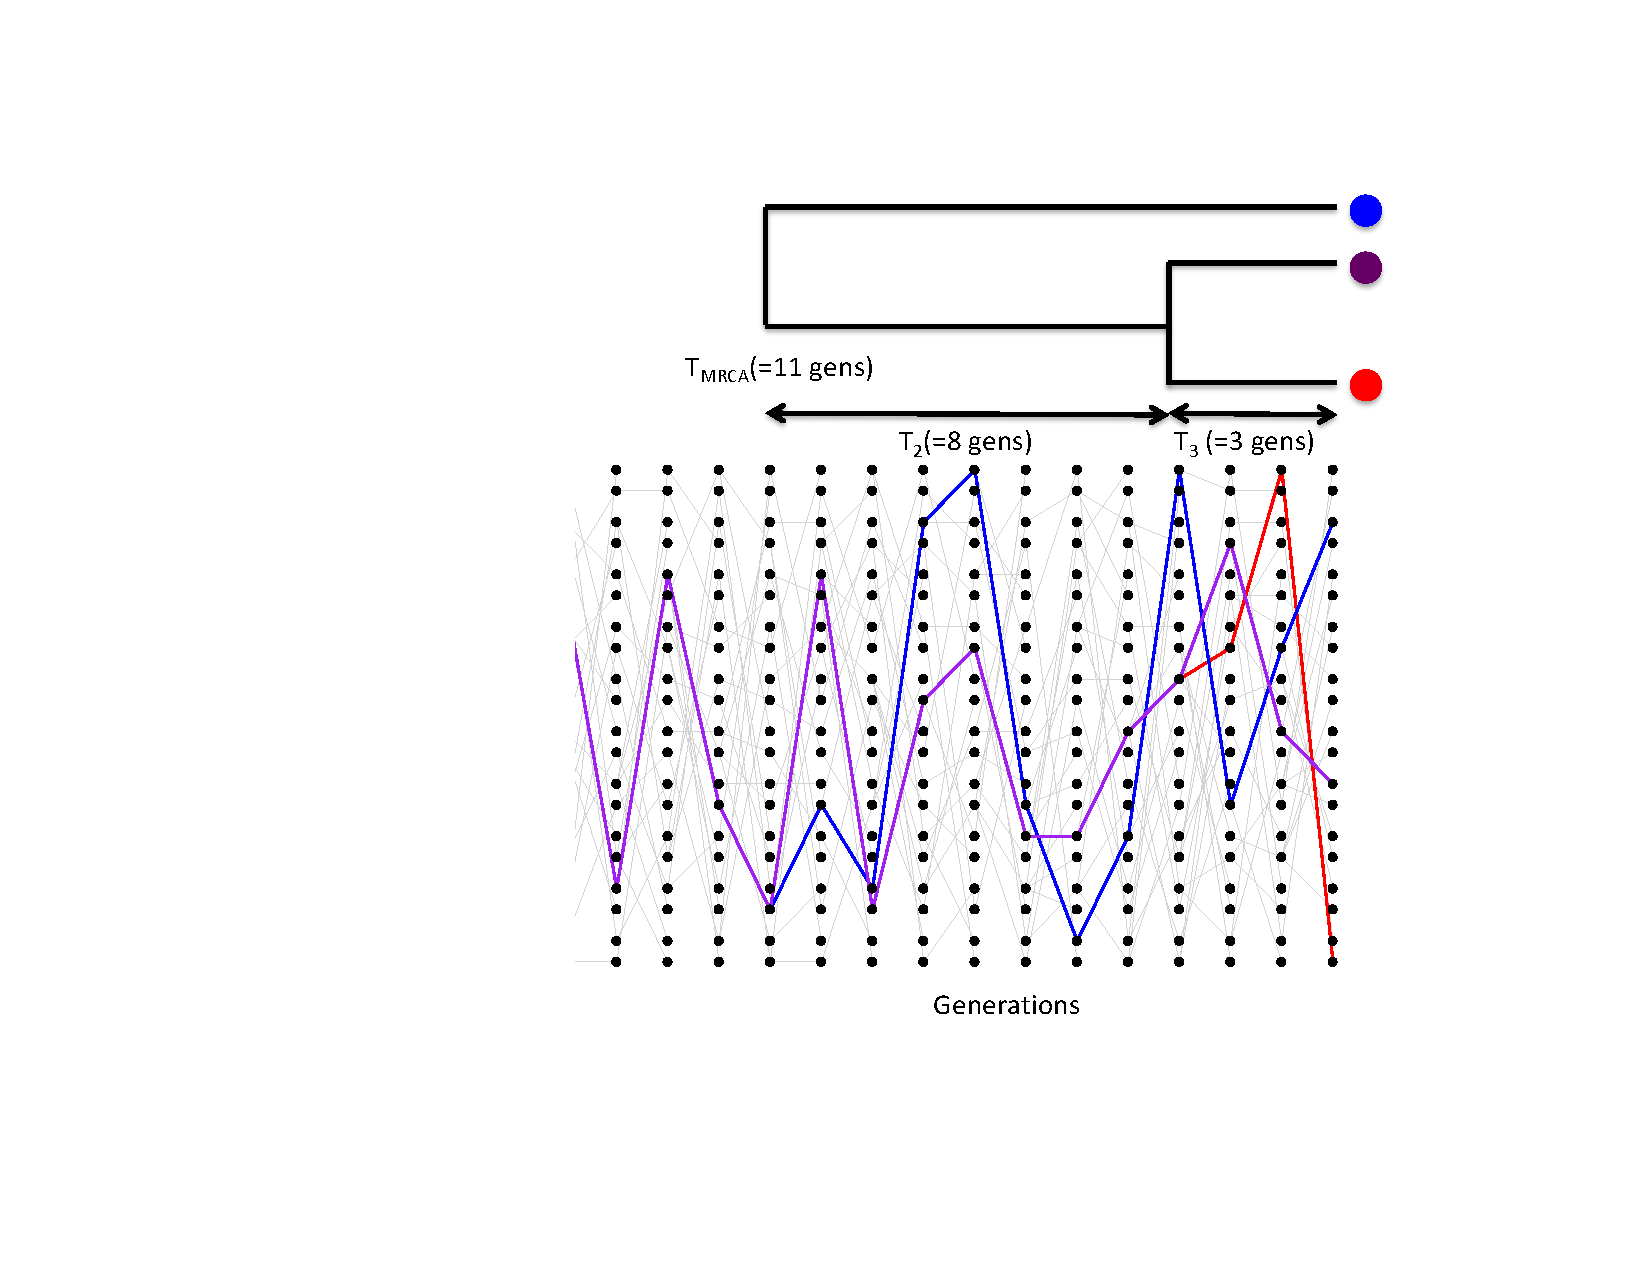
\includegraphics[width = 0.75 \textwidth]{figures/Coalescent/Coal_three_lineages.pdf}
\end{center}
\caption{A simple simulation of the coalescent process for three
  lineages. We track the ancestry of
  three modern-day alleles, the first pair (blue and purple) coalesce four generations back, after which
  there are only two independent lineages we are tracking. This pair
  then coalesces twelve generations in the past. Note that different
  random realizations of this process will differ from each other a lot. The $T_{MRCA}$ is $T_3+T_2$. The total time in the tree is $T_{tot}=3T_3 + 2T_2= 25$ generations. \gitcode{https://github.com/cooplab/popgen-notes/blob/master/Rcode/track_alleles.R} } \label{fig:Coalescent_simulation_3}
\end{figure}
%JRI: image legend has TMRCA but you don't define this term until later.

The probability that a specific pair of alleles find a common ancestor in the
preceding generation is still $\nicefrac{1}{(2N)}$. There are three possible pairs of
alleles, so the probability that no pair finds a common ancestor in the preceding generation is
\begin{equation}
\left(1-\frac{1}{2N} \right)^3 \approx \left( 1- \frac{3}{2N} \right)
\end{equation}
In making this approximation we are multiplying out the right hand-side
and ignoring terms of $1/N^2$ and higher (a Taylor approximation, see Appendix eqn \eqref{eqn:Taylor_exp}).
%JRI: isn't it the left-hand side you're multiplying out?
 See Figure \ref{fig:Coalescent_simulation_3} for a random realization of this process. \\

More generally, when we sample $i$ alleles there are ${i \choose 2}$
pairs,\sidenote{said as ``i choose 2''}  i.e. $i(i-1)/2$ pairs.
%JRI: i choose 2 is nice, but you've used the binomial coefficient previously without explaining this
Thus, the probability that no pair of alleles in a sample of size $i$ coalesces in the preceding generation is
\begin{equation}
\left(1-\frac{1}{(2N)} \right)^{{i \choose
 2}} \approx \left( 1- \frac{{i \choose
 2}}{2N}\right)
\end{equation}
while the probability any pair coalesces is $\approx \nicefrac{{i \choose
 2}}{2N}$, again using eqn \eqref{eqn:Taylor_exp}.\\

We can ignore the possibility that more than pairs of alleles (e.g. tripletons)
simultaneously coalesce at once as terms of $\nicefrac{1}{N^2}$ and higher
can be ignored as they are vanishingly rare. Obviously in reasonable
sample sizes there are many more triples (${i \choose 3}$) and higher order
combinations than there are pairs (${i \choose 2}$), but if $i \ll N$ then we are safe to
ignore these terms.


When there are $i$ alleles, the probability that we wait until the
$t+1$ generation before
any pair of alleles coalesces is
\begin{equation}
P(T_i =t+1) = \frac{{i \choose
 2}}{2N}\left( 1- \frac{{i \choose
 2}}{2N}\right)^{t} \label{eqn:T_i}
\end{equation}
Thus the waiting time to the first coalescent event while there are $i$ lineages is a geometrically distributed random variable\sidenote{see Appendix eqn \eqref{eqn:geometric_def}.}  with probability of success $p=\nicefrac{{i \choose 2}}{2N}$, which we denote by
\begin{equation}
T_i \sim \text{Geo}
\left(  \nicefrac{{i \choose
      2}}{2N} \right).
\end{equation}
The mean waiting time till any of pair within our
 sample coalesces is
\begin{equation}
\E( T_i) = \frac{2N}{{i \choose  2}}  \label{eqn:E_T_i}
\end{equation}
which again follows from the mean of a geometric random variable being $\nicefrac{1}{p}$.
\marginnote{
To see the continuous time  version of this, note that \eqref{eqn:T_i} is
\begin{equation}
\approx  \frac{{i \choose
 2}}{2N} \exp \left( - \frac{{i \choose
 2}}{2N} t \right)
\end{equation}
The waiting time $T_i$ to the first coalescent event in a sample
of $i$ alleles is thus exponentially distributed with rate $\nicefrac{{i \choose
 2}}{2N}$, i.e. $T_i \sim \text{Exp}\left(\nicefrac{{i \choose
 2}}{2N} \right)$. }
After a pair of alleles first finds a common ancestral allele some
number of generations back in the past, we only have to keep
track of that common ancestral allele for the pair when looking further into the past. Thus when a pair
of alleles in our sample of $i$ alleles coalesces, we then switch to
having to follow $i-1$ alleles back in time. Then when a pair of these $i-1$
alleles coalesce, we then only have to follow $i-2$ alleles back. This
process continues until we coalesce back to a sample of two, and from
there to a single most recent common ancestor (MRCA).\\


\paragraph{Simulating a coalescent genealogy}
To simulate a coalescent genealogy at a locus for a sample of $n$ alleles we therefore simply follow the following
algorithm:
\begin{enumerate}
\item Set $i=n$.
\item Simulate a random variable to be the time $T_i$ to the next coalescent event from $T_i \sim
  \text{Exp}\left(\nicefrac{{i \choose
 2}}{2N} \right)$
\item Choose a pair of alleles to coalesce at random from all possible
 pairs.
\item Set $i=i-1$
\item Continue looping steps 2-4 until $i=1$, i.e. the most recent
 common ancestor of the sample is found.
\end{enumerate}
By following this algorithm we are generating realizations of the
genealogy of our sample. \\



\subsection{Expected properties of coalescent genealogies and
  mutations.}

\begin{figure}
\begin{center}
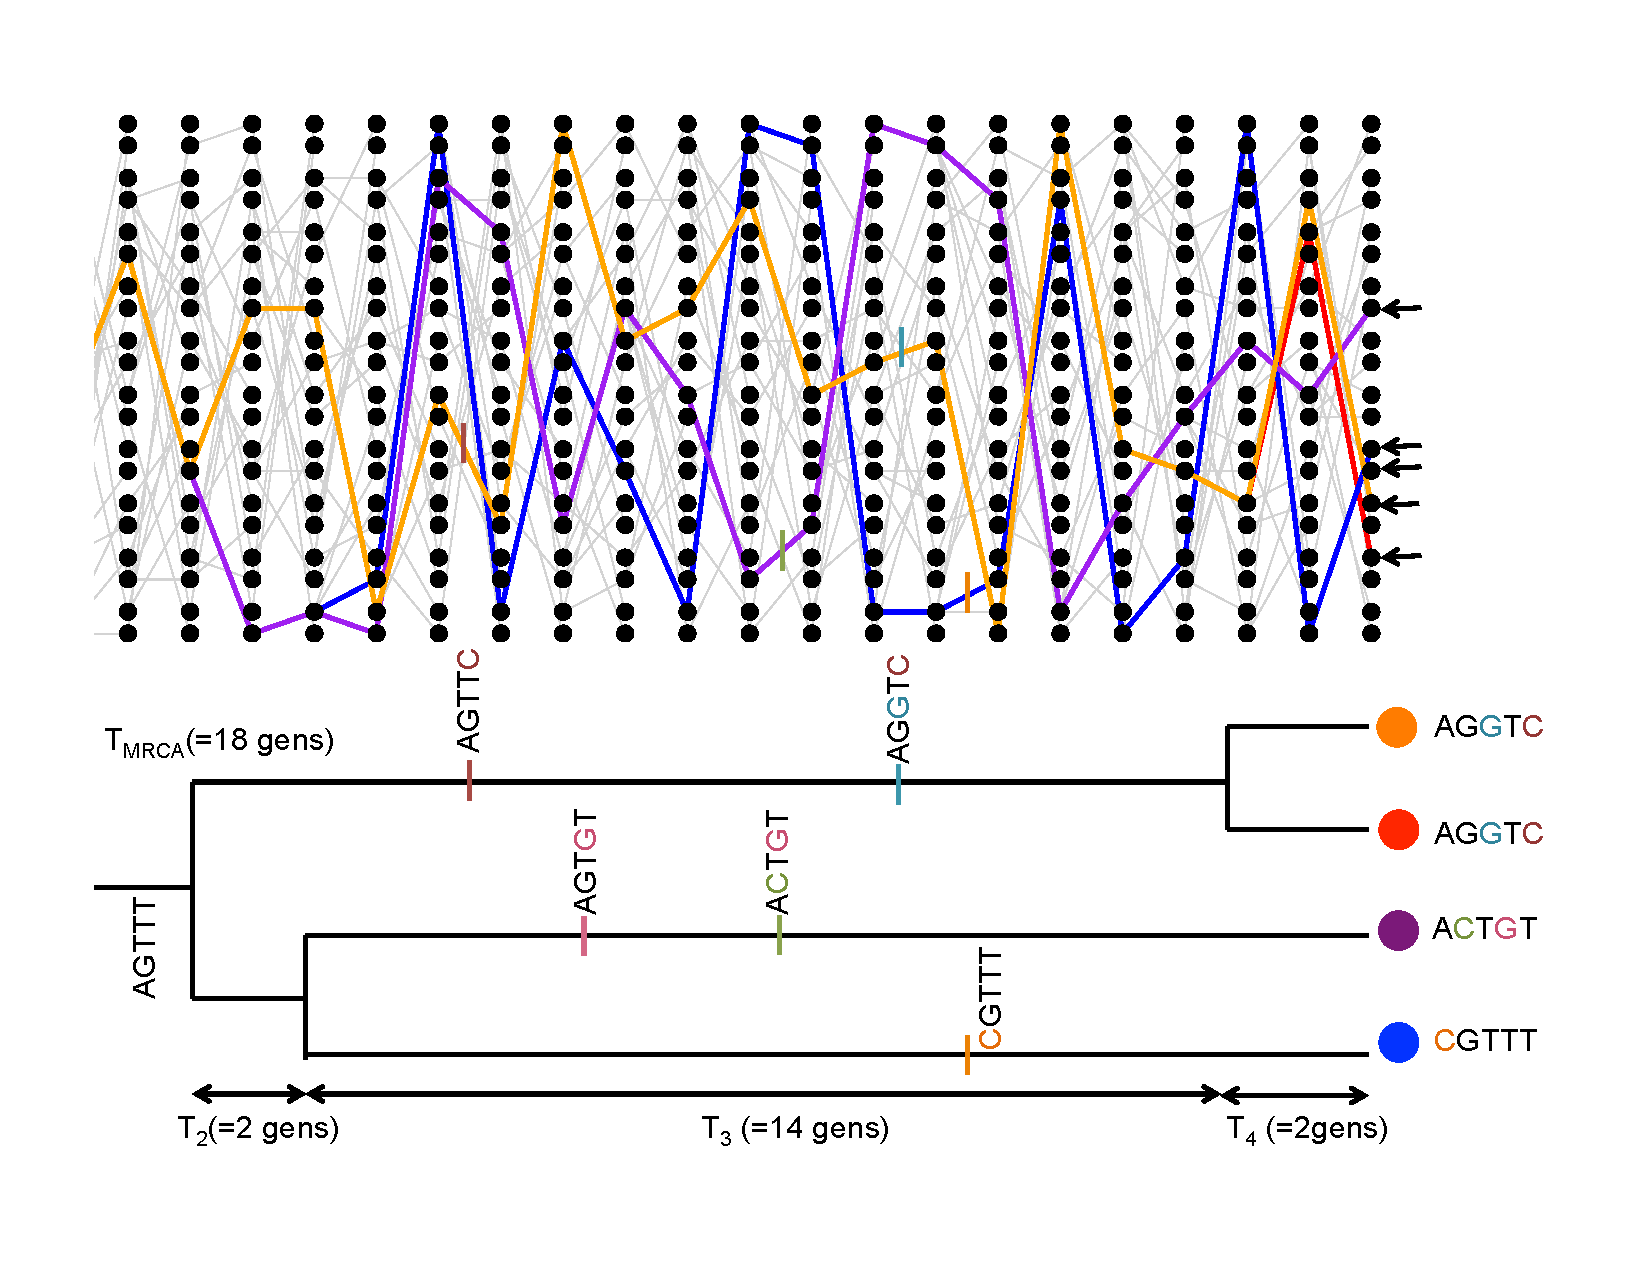
\includegraphics[width= \textwidth]{figures/Coalescent/Coal_w_muts.pdf}
\end{center}
\caption{A simple coalescent tree from a single coalescent simulation, tracing the genealogy of 4 alleles with mutational changes marked with dashes showing transitions away from the MRCA sequence (AGTTT) . The $T_{MRCA}$ is $T_4+T_3+T_2$. The total time in the tree is $T_{tot}=4 T_4+3T_3 + 2T_2= 54$ generations. \gitcode{https://github.com/cooplab/popgen-notes/blob/master/Rcode/track_alleles.R}  } \label{fig:Coal_w_muts}
\end{figure}


\paragraph{The expected time to the most recent common ancestor.}
We will first consider the time to the most recent common ancestor of
the entire sample ($T_{MRCA}$). This is
\begin{equation}
T_{MRCA} = \sum_{i=n}^2 T_i
\end{equation}
generations back, where we are summing from $i=n$ alleles counting backwards to $i=2$ alleles (see Figure \ref{fig:Coal_w_muts} for example). As our coalescent times for different $i$ are independent, the expected time to the most recent common ancestor
is
\begin{equation}
\E(T_{MRCA}) = \sum_{i=n}^2 \E(T_i) = \sum_{i=n}^2  2N/{i \choose
 2}
\end{equation}
Using the fact that $\frac{1}{i(i-1)}=\frac{1}{i-1} - \frac{1}{i}$ and a bit of
rearrangement, we can rewrite this as
\begin{equation}
\E(T_{MRCA}) = 4N\left(1- \frac{1}{n} \right) \label{TMRCA_neutral}
\end{equation}
So the average $T_{MRCA}$ scales linearly with population
size $N$. Interestingly, as we move to larger and larger samples (i.e. $n \gg 1$), the average
time to the most recent common ancestor converges on $4N$. What's
happening here is that in large samples our lineages typically coalesce rapidly
at the start and very soon coalesce down to a much smaller number of
lineages.   \\

\begin{question}
Assume an autosomal effective population of 10,000 individuals (roughly the long-term human estimate) and a generation time of 30 years. What is the expected time to the most recent common ancestor of a sample of 20 people? What is this time for a sample of 500 people?
\end{question}
\paragraph{The expected total time in a genealogy and the number of
  segregating sites.}

Mutations fall on specific lineages of the coalescent genealogy and are transmitted to all descendants of their lineage. Furthermore, under the infinitely-many-sites assumption, each mutation creates a new segregating site. The mutation process is a
\emph{Poisson process}, and the longer a particular lineage, i.e. the more generations of meioses it represents, the more
mutations that can accumulate on it. The total number of segregating sites in
a sample is thus a function of the \emph{total} amount of time in the
genealogy of the sample, or the sum of all the branch lengths on the genealogical tree,
$T_{tot}$. Our total amount of time in the genealogy is

\begin{equation}
T_{tot} = \sum_{i=n}^2 iT_i
\end{equation}
as when there are $i$ lineages, each contributes a time $T_i$ to the total time (see Figure \ref{fig:Coal_w_muts} for an example). Taking the expectation of the total time in the genealogy,
\begin{equation}
\E(T_{tot}) = \sum_{i=n}^2 i \frac{2N}{{i \choose
 2} } = \sum_{i=n}^2 \frac{4N}{i -1} =\sum_{i=n-1}^1 \frac{4N}{i} \label{eqn:E_T_tot}
\end{equation}
we see that our expected total amount of time in the genealogy scales linearly
with our population size $N$. Our expected total amount of time is also
increasing with sample size $n$, but is doing so very slowly. %To see this
%more carefully, we can see that for large $n$
%\begin{equation}
%\E(T_{tot}) = \sum_{i=n-1}^1 \frac{4N}{i}
%\end{equation}
\marginnote{To get a better sense of how $T_{tot}$ grows with the sample size, we
  can approximate the sum \ref{eqn:E_T_tot} by an integral, which will work for large $n$. The result is  $\int_1^{n-1} \frac{4N}{i} di
= 4N \log(n-1)$. }
This again follows
from the fact that in large samples, the initial coalescence usually
happens very rapidly, so that extra samples add little to the total
amount of time in the genealogical tree. \\

We saw above that the number of mutational differences between a pair
of alleles that coalescence $T_2$ generations ago was Poisson with a
mean of $2 \mu T_2$, where $2T_{2}$ is the total branch length in this simple 2-sample genealogical tree. A mutation that occurs on any branch of our
genealogy will cause a segregating polymorphism in the sample
(meeting our infinitely-many-sites assumption). Thus, if the total time
in the genealogy is $T_{tot}$, there are $T_{tot}$
generations for mutations. So the total number of mutations
segregating in our sample ($S$) is Poisson with mean $\mu T_{tot}$. Thus the
expected number of segregating  sites in a sample of size $n$ is
\begin{equation}
\E(S) = \mu \E(T_{tot}) = \sum_{i=n-1}^1 \frac{4N\mu }{i} = \theta
\sum_{i=n-1}^1 \frac{1}{i}
\end{equation}
Note that this is growing with the sample size $n$, albeit very slowly (roughly at the rate of the $\log$ of the sample size).
We can use this formula to derive another estimate of the population scaled mutation rate $\theta$, by setting our observed number of segregating sites in a sample ($S$) equal to this expectation. We'll call this estimator $\widehat{\theta}_W$:
\begin{equation}
\widehat{\theta}_W =\frac{ S}{\sum_{i=n-1}^1 \nicefrac{1}{i}}   \label{watterson_theta}
\end{equation}
This estimator of $\theta$ was devised by \citet{watterson:75}, hence the $W$.


\paragraph{The neutral site-frequency spectrum.}

We can use our coalescent process to find the expected number of
derived alleles present $i$ times out of a sample size $n$, e.g. how many singletons ($i = 1$) do we
%JRI: have you defined ``derived''?
expect to find in our sample? For example, in Figure \ref{fig:Coal_w_muts} in our sample of four sequences, there are 3 singletons and 2 doubletons. The number of sites with these different allele frequencies depends on the lengths of specific genealogical branches. A mutation that falls on a branch with $i$ descendants will create a derived allele with frequency $i$. For example, in our example tree  in Figure \ref{fig:Coal_w_muts}, the total number of generations where a mutation could arise and be a doubleton is $T_3+2T_2$, the total length of the branch ancestral to just the orange and red allele $(T_3+T_2)$ plus the branch ancestral to just the blue and purple allele $(T_2)$.
%JRI: this explanation is fine, but it's next to the figure below and I spent 30 seconds trying to figure out why you were multiplying T2 by 2 before I realized this figure wasn't mentioned until next page.

\begin{marginfigure}[-4cm]
\begin{center}
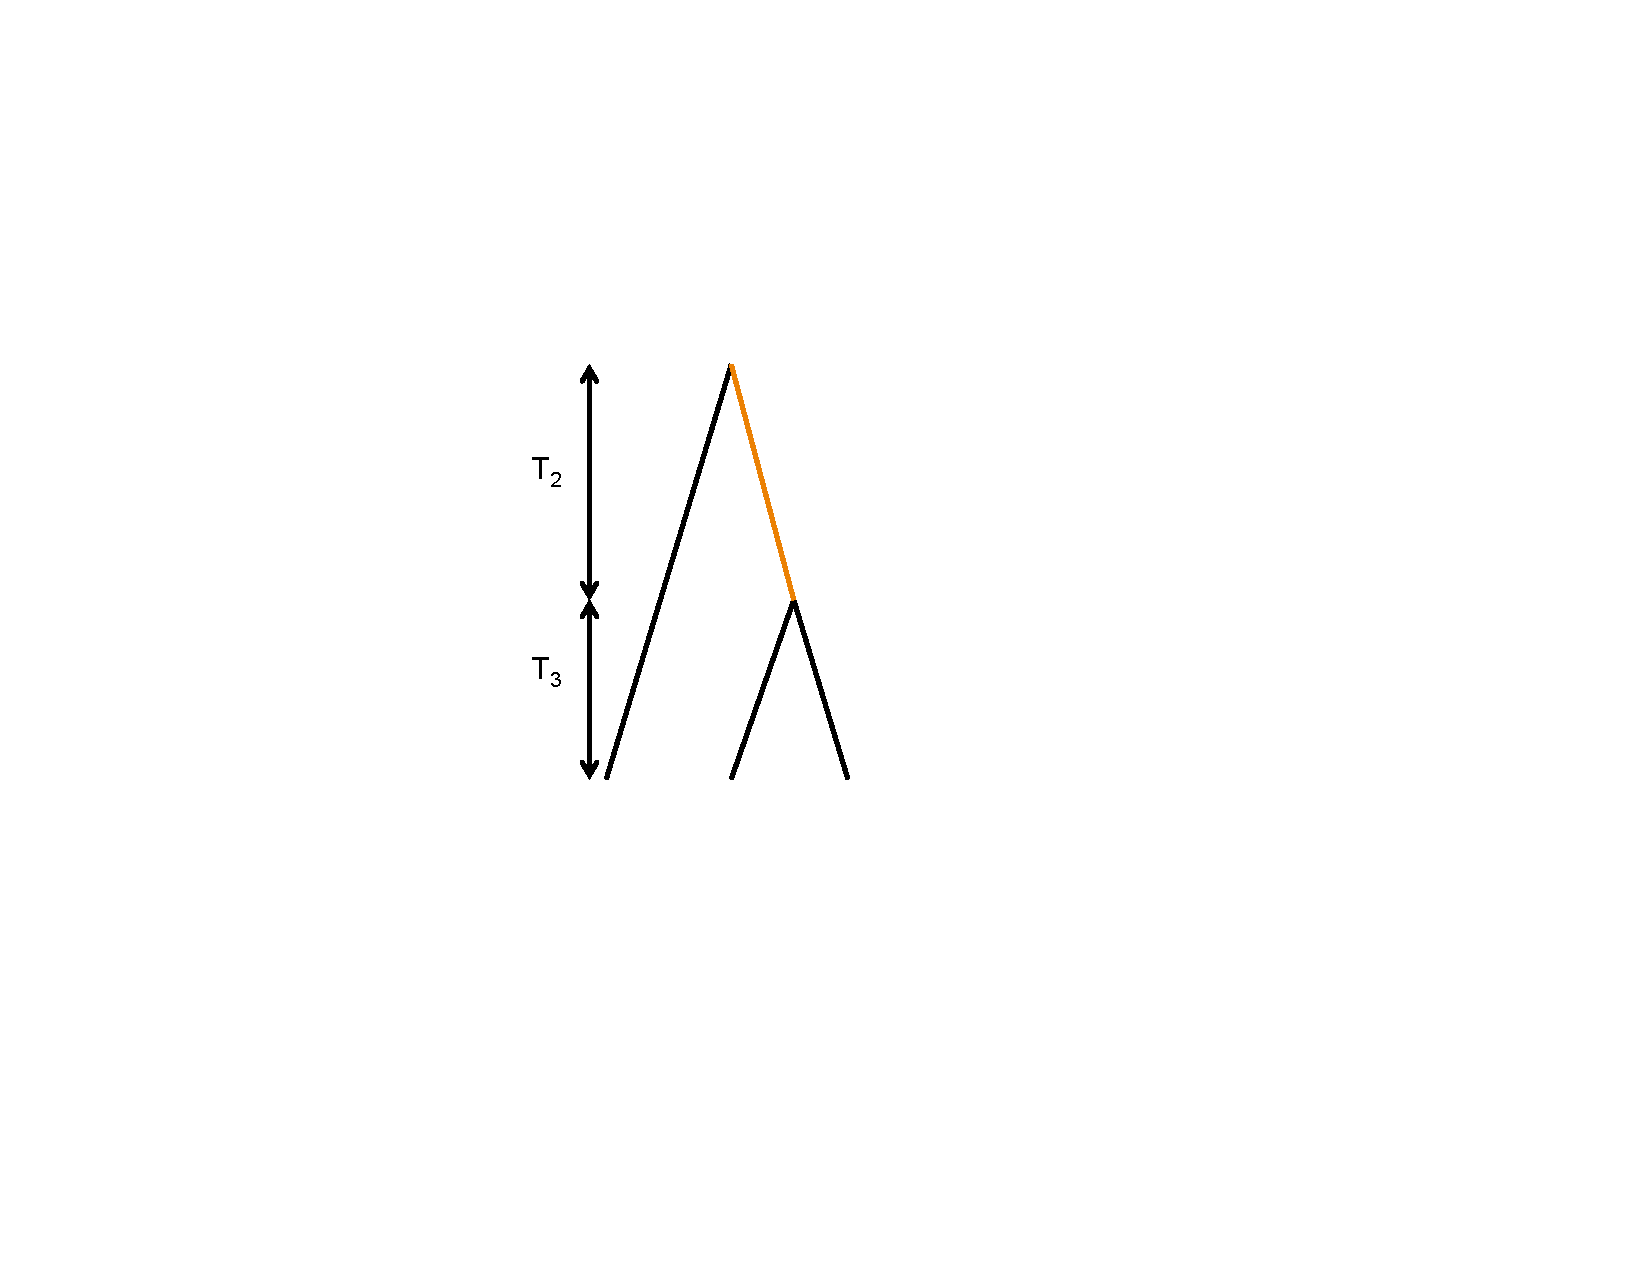
\includegraphics[width= \textwidth]{figures/Genetic_drift/freq_spec_tree.pdf}
\end{center}
\caption{A tree for three samples; note that this is the only possible
tree shape (treating the tips as unlabeled, i.e.  I don't care which pair of sequences carry a doubleton, just that any two sequences carry a derived allele).} \label{fig:freq_coal}
\end{marginfigure}

To see how we could go about working this out, lets start by considering the simple coalescent tree, shown in Figure \ref{fig:freq_coal}, for sample of $3$ alleles drawn from a population. Mutations that fall on the
branches coloured in black will be derived singletons, while mutations that
fall along the orange branch will be doubletons in the sample. The
total number of generations where a singleton mutation could arise is
$3 T_3 + T_2$. Note that we only count the time where there are two
lineages $(T_{2})$ once. So our expected number of singletons, using eqn \eqref{eqn:E_T_i}, is
\begin{equation}
\E(S_i) = \mu \left( 3\E(T_3) +  \E(T_2) \right) = \mu \left( 3
  \frac{2N}{3}+ 2N \right) = \theta
\end{equation}
By similar logic, the time where doubletons could arise is
$T_2$ and our expected number of doubletons is $\E(S_i)
=\theta/2$. Thus, there are on average half as many doubletons as singletons.

Extending this logic to larger samples might be doable, but is tedious (I mean really tedious: for 10 alleles there are thousands of possible tree shapes and the task quickly gets impossible even computationally). A nice, relatively simple proof of the neutral site frequency spectrum is given by
\citep{Hudson:15}, but we won't give this here. The general form is:
\begin{equation}
\E(S_i) = \frac{\theta }{i}   \label{eqn:neutral_freq_spec}
\end{equation}
i.e. there are twice as many singletons as doubletons, three times as many
singletons as tripletons, and so on. The other thing that will be
helpful for us to know is that neutral alleles at intermediate frequency tend to be old, and those that are rare in the sample are young. We expect to see a lot more rare alleles in our sample than common alleles.

\begin{question}
There are two possible tree shapes that could relate four
samples. Draw both of them and separately colour (or otherwise mark) the branches by where singletons, doubletons, and tripleton derived alleles could arise.
%{\bf A)}
%{\bf B)} Can you work out the expected number of each allele count? [{\bf OPTIONAL}] \erin{change for different tree question}
\end{question}

We can also ask the probability of observing a derived allele segregating at frequency $i/n$ given that the site is polymorphic in our sample of size $n$ (i.e. given that $0<i<n$ ). We can obtain this probability by dividing the expected number of sites segregating for an allele at frequency $i$ by the expected number segregating at all of the possible allele frequencies for polymorphisms in our sample
\begin{eqnarray}
P(i |0<i<n) &=\frac{\E(S_i)}{\sum_{j=1}^{n-1} \E(S_j)} = \frac{\nicefrac{1}{i}}{\sum_{j=1}^{n-1} \nicefrac{1}{j}}.
\end{eqnarray}
We can interpret this probability as the fraction of polymorphic sites we expect to find at a frequency $i/n$.

\paragraph{Tests based on the site frequency spectrum}
Population geneticists have proposed a variety of ways to test whether an observed site frequency spectrum conforms to its
neutral, constant-size expectations. These tests are
useful for detecting population size changes using data across many loci, or
for detecting the signal of selection at individual loci. One of
the first tests was proposed by \citep{tajima:89}, and is called
Tajima's $D$. Tajima's $D$ is
\begin{equation}
  D = \frac{\hat{\theta}_{\pi}-\hat{\theta}_{W}}{C} \label{eqn_Tajimas_D}
\end{equation}
where the numerator is the difference between the estimate of
$\theta$ based on pairwise differences and that based on segregating
sites. As these two estimators both have expectation $\theta$ under
the neutral, constant-size model, the expectation of $D$ is zero. The denominator $C$ is a positive constant; it's the square-root of an estimatorof the variance of this difference under the constant population size, neutral model. This constant was chosen for $D$ to have mean zero and variance $1$ under the null model, so we can test for  departures from this simple null model.\\

An excess of rare alleles compared to the constant-size, neutral
model will result in a negative Tajima's $D$, because each
additional rare allele increases the number of segregating sites by
$1$, but only has a small effect on the number of pairwise differences between samples.
In contrast, a positive Tajima's $D$ reflects an excess of intermediate frequency alleles relative to the constant-size, neutral expectation. Alleles at intermediate-frequency increase pairwise diversity
more per segregating site than typical, thus increasing $\theta_{\pi}$ more than $\theta_{W}$.

\subsection{Demography and the coalescent}

\begin{marginfigure}
\begin{center}
  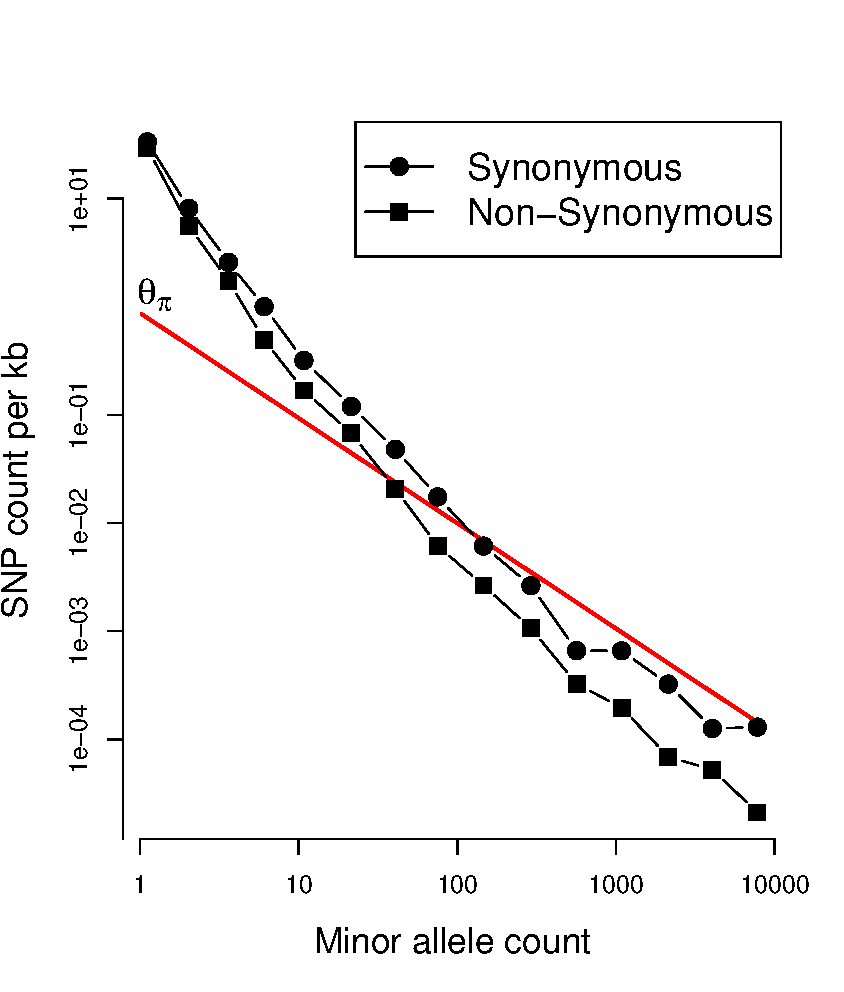
\includegraphics[width = \textwidth]{Journal_figs/genetic_drift/human_pop_growth/Nelson_pop_growth.pdf}
\end{center}
\caption{Data from 202 genes from 14002 people of European ancestry (28004 alleles). Note
  the double log-scale. The red
  line gives the neutral, constant population size estimate of the site frequency spectrum, our equation \eqref{eqn:neutral_freq_spec}, using a  $\theta$ estimated from $\pi$. Note how the non-synonymous changes are even more skewed towards rare alleles, likely due to selection against non-synonymous alleles preventing them from reaching high frequency. Data from \citet{nelson:12}. \gitcode{https://github.com/cooplab/popgen-notes/blob/master/Journal_figs/genetic_drift/human_pop_growth/Nelson_pop_growth.R} } \label{fig:Human_growth}
\end{marginfigure}
We've already seen how changes in population size can change the rate
at which heterozygosity is lost from the population (see the
discussion around eqn. \eqref{eqn:var_pop_coal}). If the population
size in generation $i$ is $N_i$, the probability that a pair of
lineages coalesce is $\nicefrac{1}{(2N_i)}$; this conforms to our
intuition that if the population size is small, the rate at which
pairs of lineages find their common ancestor is faster. We can potentially accommodate rapid random fluctuations in population size by simply using the effective population size $N_e$ in place of $N$. However,
longer term more systematic changes in population size will distort
the coalescent genealogies, and hence patterns of diversity, in more
systematic ways.

We can see how demography potentially distorts the observed frequency spectrum away from the neutral expectation in a very large sample of humans shown in Figure \ref{fig:Human_growth}. For
comparison, the neutral frequency spectrum, eqn
\eqref{eqn:neutral_freq_spec}, is shown as a red line. There are
  vastly more rare alleles than expected under our neutral, constant-size-size model, but the neutral prediction and reality agree somewhat more for alleles that are more common.

\begin{figure*}
\begin{center}
  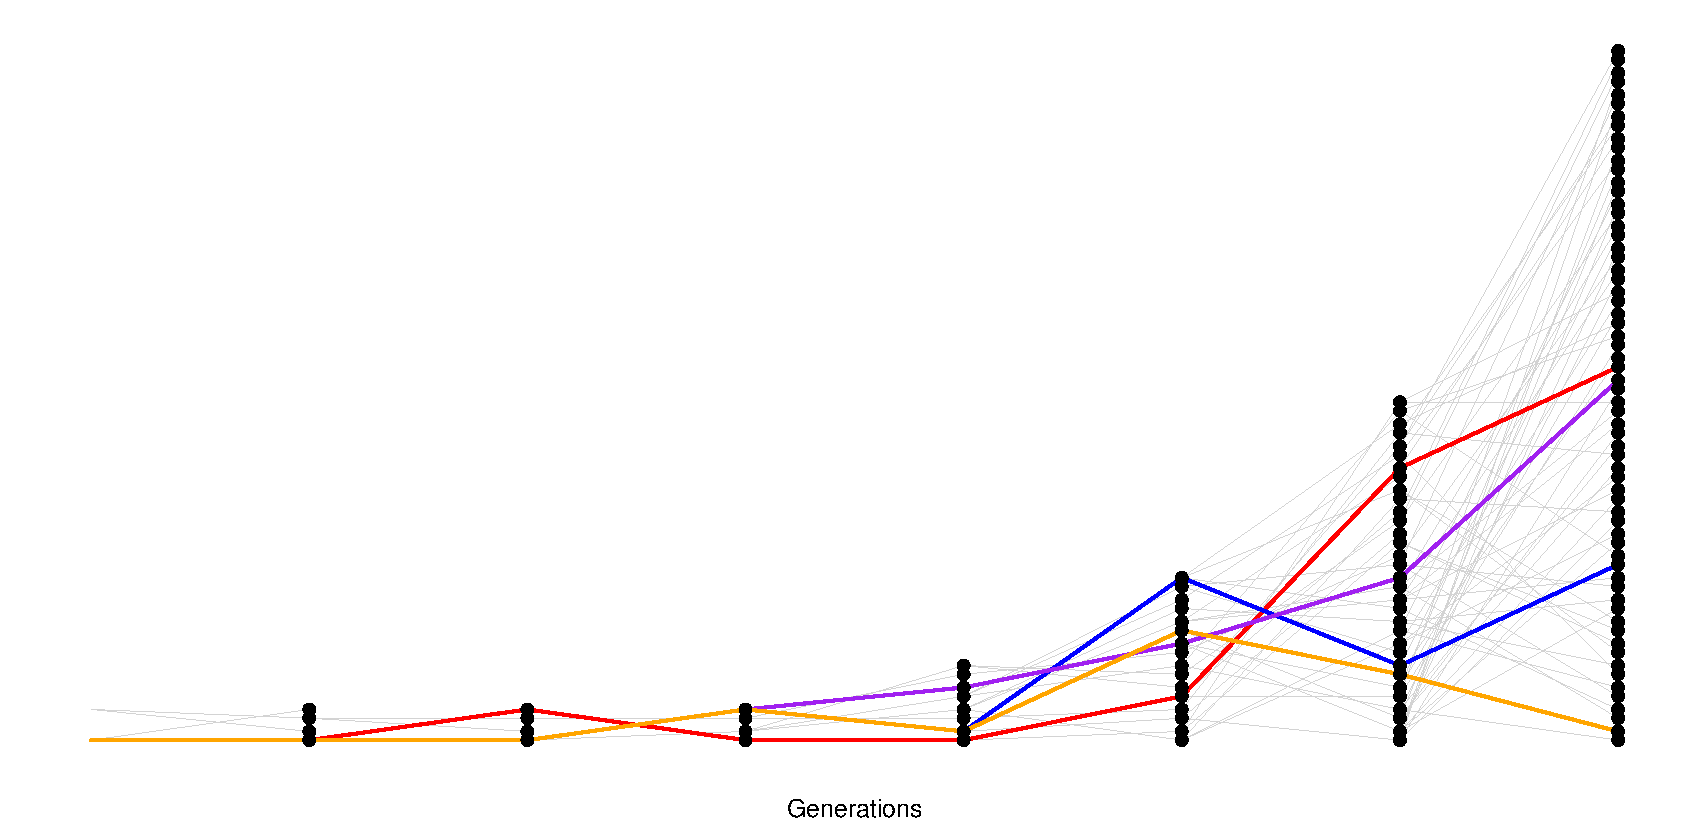
\includegraphics[width = \textwidth]{figures/Genetic_drift/Demography/Growth_genealogy.pdf}
\end{center}
\caption{A realization of the coalescent process in a growing population. The population underwent a period of doubling every generation. The initial population size of just two individuals, maintained for a number of generations, is obviously highly unrealistic but serves our purpose. \gitcode{https://github.com/cooplab/popgen-notes/blob/master/Rcode/track_alleles.R}  } \label{fig:Genealogy_growth}
\end{figure*}
%JRI: I realize this contrasts with the later bottleneck figure, but I just don't like this one very much. I don't find it very useful as it's hard to distinguish the differences in rates of coalescence from stochastic differences in other similar figures. I'd be tempted to remove this but keep the later bneck paper. Perhaps if you want interestd students to be able to play with it link to a larger version or just the code?

Why is this? Well, these patterns are likely the result of the very recent
explosive growth in human populations. If the population has grown rapidly, then the pairwise-coalescent rate in the past may be much higher than the coalescent rate closer to the present. (see Figure \ref{fig:Genealogy_growth}).

One consequence of a recent population expansion is that there is much less genetic diversity in the population than you'd predict using the census
population size. Humans are one example of this effect; there are $7$ billion
of us alive today, but this is due to very rapid population growth
over the past thousand to tens of thousands of years. Our level of
genetic diversity is very much lower than you'd predict given our
census size, reflecting our much smaller ancestral population. A second consequence of recent population expansion is that the deeper coalescent branches are much more squished together in time compared to those in a constant-sized population.  Mutations on deeper branches are the source of alleles at more intermediate frequencies, and so there are even fewer intermediate-frequency alleles
in growing populations. That's why there are so many rare alleles,
especially singletons, in this large sample of Europeans.


Another common demographic scenario is a population bottleneck. In a bottleneck, the population size crashes dramatically, and subsequently
recovers. For example, our population may have had size $N_{\textrm{Big}}$
and crashed down to $N_{\textrm{Small}}$. One example of a
bottleneck is shown in Figure \ref{fig:Genealogy_crash}.
\begin{figure*}
\begin{center}
  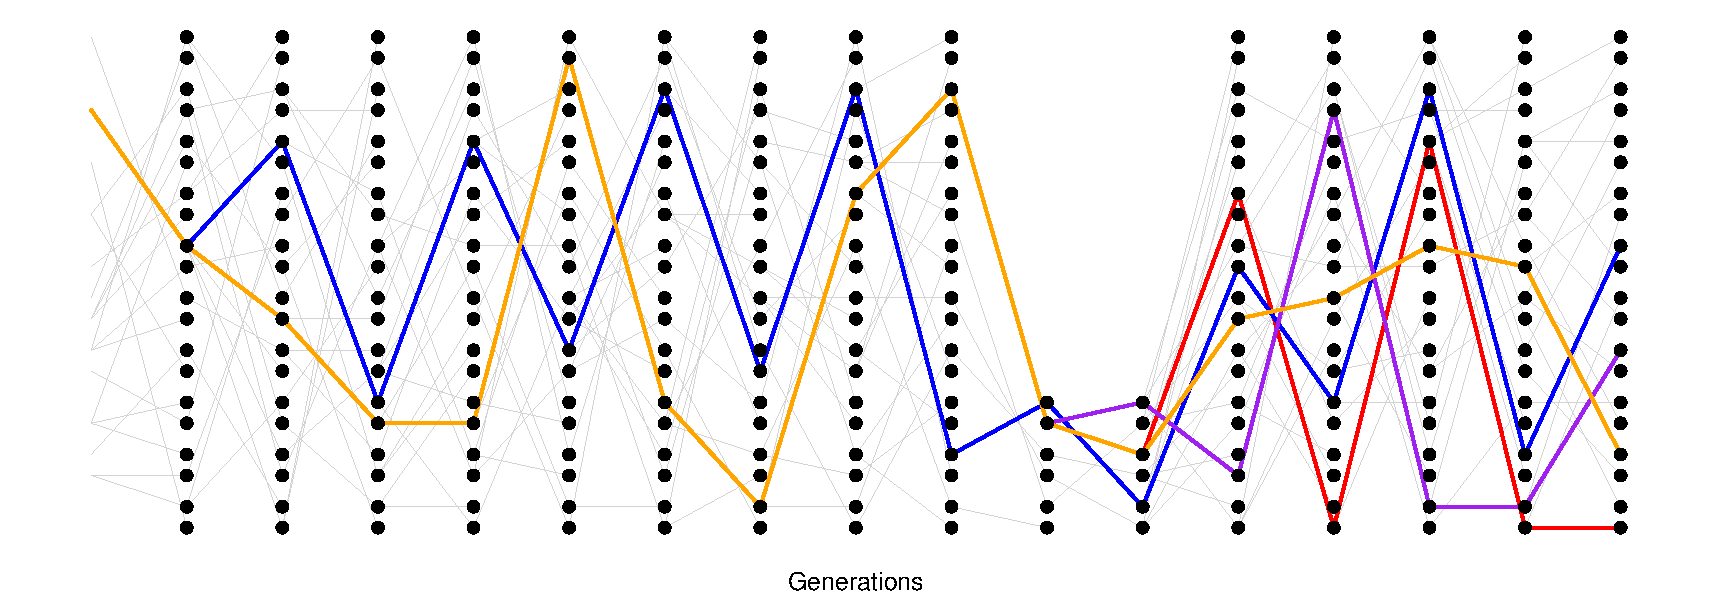
\includegraphics[width = \textwidth]{figures/Genetic_drift/Demography/Crash_genealogy.pdf}
\end{center}
\caption{A realization of the coalescent process in a bottlenecked population. Our population under went a bottleneck eight generations in the past. \gitcode{https://github.com/cooplab/popgen-notes/blob/master/Rcode/track_alleles.R} } \label{fig:Genealogy_crash}
\end{figure*}
Looking at a sample of lineages drawn from the population today, if
the bottleneck was somewhat recent ($\ll N_{\textrm{Big}}$ generations
in the past) many of our lineages will not have coalesced before reaching
the bottleneck, moving backward in time. But during the bottleneck our
lineages coalesce at a much higher rate, such that many of our
lineages will coalesce if the bottleneck lasts long enough
($\sim N_{\textrm{Small}}$ generations). If the bottleneck is very
strong, then all of our lineages will coalesce during the bottleneck, and the resulting site frequency spectrum may
look very much like our population growth model (i.e. an excess of rare
alleles). However, if some pairs of lineages escape coalescing during
the bottleneck, they will coalesce much more deeply in time (e.g. the
blue and orange ancestral lineages in
\ref{fig:Genealogy_crash}).
\begin{figure}
\begin{center}
  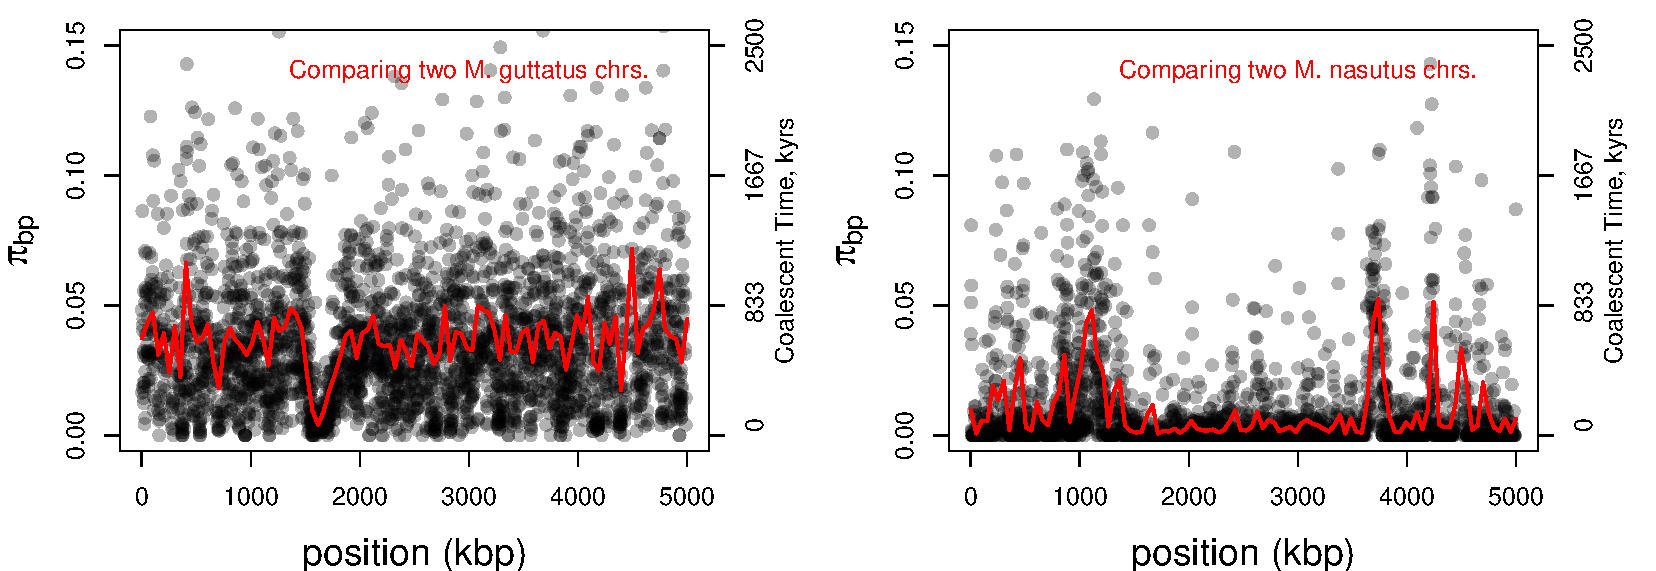
\includegraphics[width = \textwidth]{figures/Genetic_drift/Demography/Mimulus_coalescent_times.pdf}
\end{center}
\caption[][1cm]{Diversity along a region of the Mimulus genome. Black dots give $\pi$ in 1kb windows between chromosomes sampled from two individuals, the red line is a
  moving average (data from  \citeauthor{brandvain:14}). Pairwise coalescent times ($t$) estimated assuming $t= \nicefrac{\pi}{2 \mu} $ using $\mu_{BP}=10^{-9}$. \gitcode{https://github.com/cooplab/popgen-notes/blob/master/Rcode/Mimulus_coalescent_times.R} } \label{fig:Mimulus_bottleneck}
\end{figure}

An example of this is shown Figure
\ref{fig:Mimulus_bottleneck}, data from \citeauthor{brandvain:14}. {\it Mimulus nasutus} is a selfing
species that arose recently from an out-crossing progenitor {\it M.
  guttatus}, and experienced a strong bottleneck. {\it M. guttatus} has very high levels of genetic diversity
($\pi=4\%$ at synonymous sites), but {\it M. nasutus} has lost much
of this diversity ($\pi =1\%$). Looking along the genome, between a
pair of {\it M. guttatus} chromosomes, levels of
diversity are fairly uniformly high.
\begin{marginfigure}[2cm]
\begin{center}
  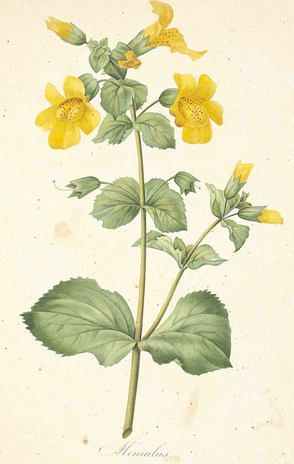
\includegraphics[width = 0.75 \textwidth]{illustration_images/Genetic_drift/Mimulus/Mimulus.png}
\end{center}
\caption{Yellow Monkeyflower {\it M. guttatus}. \newline \noindent \tiny{ Choix des plus belles fleurs et des plus beaux fruits. Pierre-Joseph
  Redout\'e. (1833). Contributed to \href{https://www.flickr.com/photos/swallowtailgardenseeds/14479197839/in/photolist-o4tF54-od9My9-odbSn4-r7eVtm-qrR4xf-x4XVdi-owo7PM-r5mart-roPqqi-owrprg-qsfzJv-wMDeSy-oupCu9-oeSX38-odaeHf-ovbTTS-roEdyK-tCQBqn-odwyWa-otAUPX-oePwpE-odca2V-tBxNdi-roL99F-odbN4q-ot1HNN-ouhP5r-odcvRH-oveh86-rpAnnD-roE9j9-rowiBc-osDEHS-od7QxD-oeQ9yS-odatza-ox9fq8-oujGWa-osBqTm-ovoAKj-r5qRxT-oeRVxu-oux9q2-tMvxm3-x5pLez-owuL1t-oePFVJ-ov1yHY-oeWskU-tmeZzB}{Flickr} by Swallowtail Garden Seeds. Public Domain.}} \label{fig:monkeyflower}  %é
\end{marginfigure}

 But in comparing two {\it
  M. nasutus} chromosomes, diversity is low because the pair of lineages generally coalesce
recently. Yet in a few places we see levels of diversity comparable to
{\it M. guttatus}; these regions correspond to genomic sites where our pair of lineages
fail to coalesce during the bottleneck and subsequently coalesce
much more deeply in the ancestral {\it M. guttatus} population.
\begin{figure}
\begin{center}
  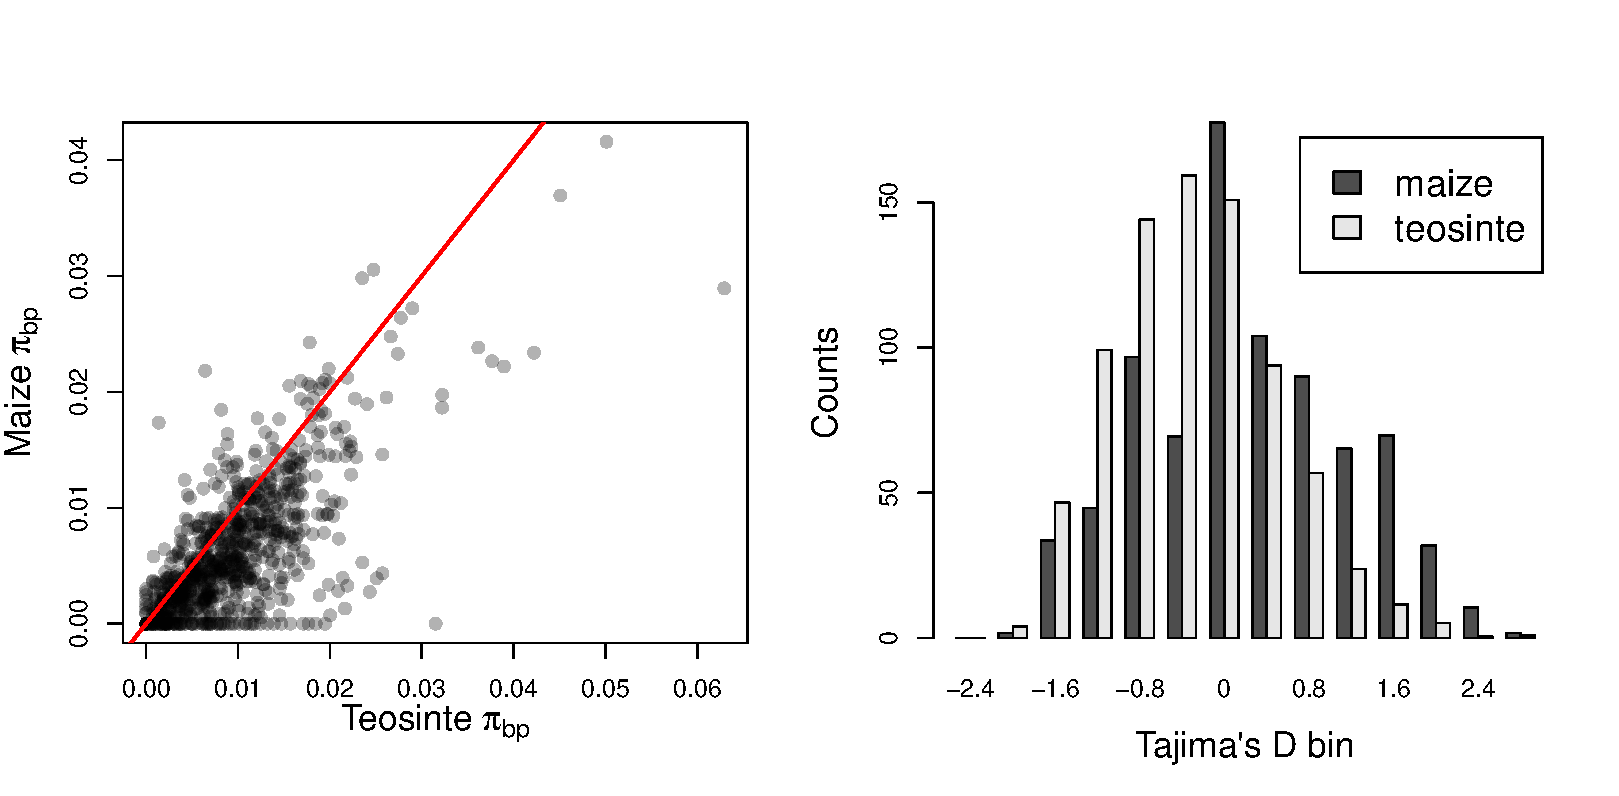
\includegraphics[width = \textwidth]{Journal_figs/genetic_drift/Maize_bottleneck/Wright_Tajima_D.pdf}
\end{center}
\caption[][-2cm]{Data for polymorphism from Maize and Teosinite: 774
  loci from \citet{Wright:05}. {\bf Left)} Genetic  diversity levels in maize and and teosinte samples at each of these loci.
Note how diversity levels are lower in maize than teosinte, i.e. most
points are below the red $x=y$ line. {\bf Right)} The distribution of Tajima's D in maize and teosinte, see how the maize distribution is shifted towards positive values. \gitcode{https://github.com/cooplab/popgen-notes/blob/master/Journal_figs/genetic_drift/Maize_bottleneck/Wright_Tajima_D.R} } \label{fig:maize_Tajimas_D}  %é
\end{figure}

 \begin{marginfigure}[4cm]
 \begin{center}
   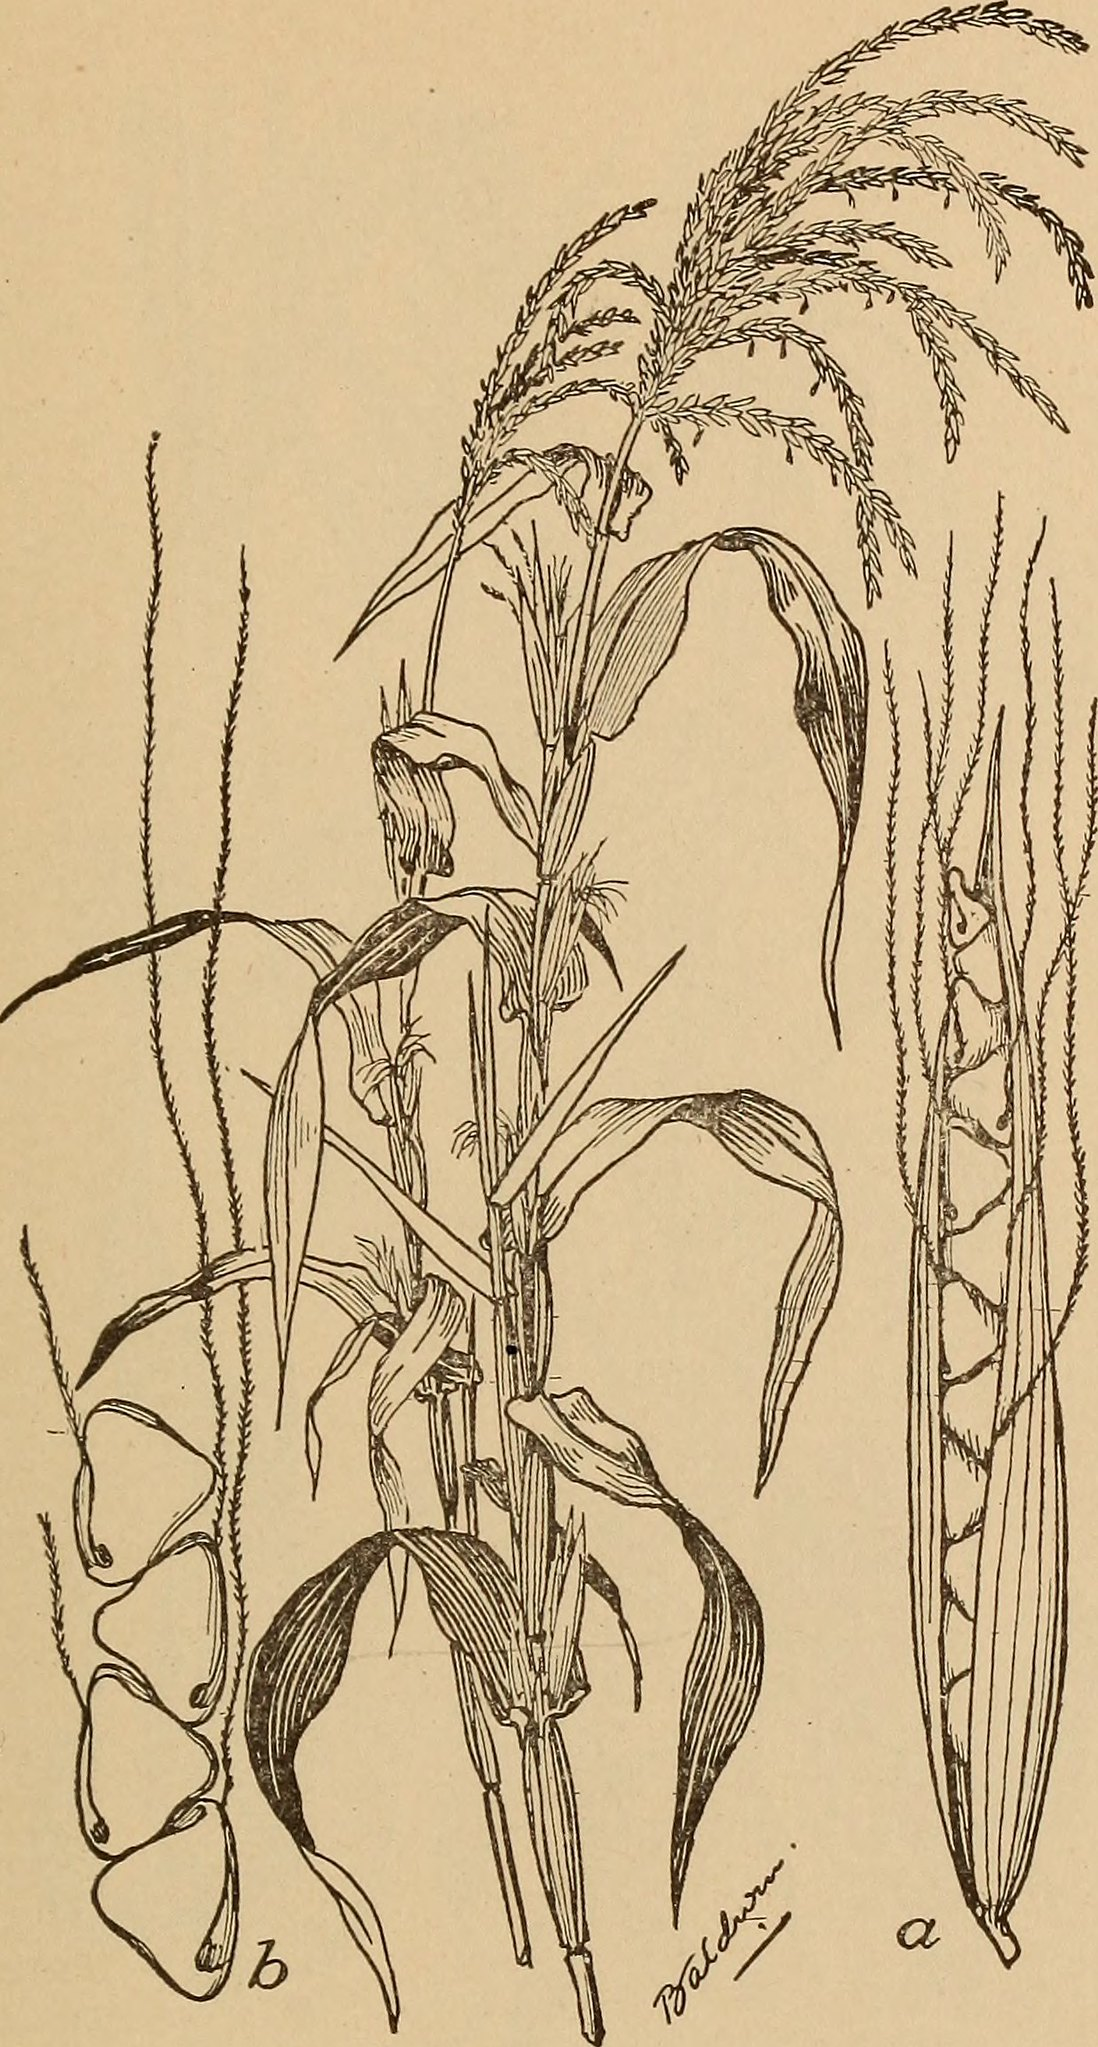
\includegraphics[width = 0.7 \textwidth]{illustration_images/Genetic_drift/teosinte/17960129408_21ad0a16f7_k.jpg}

 \end{center}
 \caption{ Teosinite ({\it Zea mays} ssp. {\it  mexicana}) \BHLNC{American grasses (1897). Scribner, FL}{https://www.flickr.com/photos/internetarchivebookimages/17960129408/}{Smithsonian Libraries}} \label{fig:Teosinite}  %é
 \end{marginfigure}  %%possible different fig https://peerj.com/preprints/26502.pdf from Jeff's paper

Mutations that arise on deeper lineages will be at intermediate frequency in our sample, and so mild bottlenecks
can lead to an excess of intermediate frequency alleles compared to
the standard constant-size model. This can skew
Tajima's D (see eqn \ref{eqn_Tajimas_D}) towards positive values and away from its expectation of
zero. One example of this skew is shown in Figure
\ref{fig:maize_Tajimas_D}. Maize ({\it Zea mays} subsp. {\it mays}) was domesticated from its wild progenitor teosinte ({\it Zea mays
subsp. parviglumis}) roughly ten thousand years ago. We can see how the
 bottleneck associated with domestication has resulted in a loss of genetic diversity in maize compared to teosinte, and the polymorphism that remains is somewhat skewed towards intermediate frequencies resulting in more positive values of Tajima's D.

\begin{question}
\citet{voight2005interrogating} sequenced 40 autosomal regions from 15 diploid samples of Hausa people from Yaounde, Cameroon. The average length of locus they sequenced for each region was $2365$bp. They found that the average number of segregating sites per locus was $S= 11.1$ and the average $\pi = 0.0011$ per base over the loci. Is Tajima's D positive or negative? Is a demographic model with a bottleneck or growth more consistent with this result?
\end{question}


\graham{Change this over to data from https://www.nature.com/articles/s41559-018-0496-4 Figure 1 for farmers and hunter-gatherers?}
